\chapter{Prezentacja warstwy użytkowej projektu}
\label{cha:prezentacja}


Warstwa użytkowa aplikacji \texttt{YLO GradeBook} została opracowana z myślą o intuicyjności, estetyce oraz ergonomii użytkowania. Interfejs powstał przy użyciu technologii \textbf{JavaFX}, a do jego definiowania wykorzystano pliki \textbf{FXML}, co umożliwiło czytelne oddzielenie logiki od prezentacji. W projekcie zastosowano również kaskadowe arkusze stylów CSS w celu zdefiniowania wyglądu widoków.

W tym rozdziale zaprezentowano strukturę graficzną głównych widoków aplikacji wraz z opisem funkcji dostępnych dla poszczególnych ról użytkownika (uczeń/nauczyciel). Dodatkowo omówiono styl graficzny interfejsu (kolorystyka, czcionki, ikony) oraz zastosowane mechanizmy wspomagające interakcję z systemem (komunikaty, formularze, walidacja danych).

\section{Opis szaty graficznej interfejsu}
Zastosowana kolorystyka interfejsu opiera się na stonowanej palecie odcieni niebieskiego, bieli i jasnej szarości, co sprzyja przejrzystości i komfortowi wizualnemu użytkownika. Dominujące barwy zostały dobrane w taki sposób, aby nie rozpraszać, a jednocześnie nadawać aplikacji nowoczesny i estetyczny wygląd.

\begin{itemize}
    \item \textbf{rgb(3,134,238)} — intensywny niebieski wykorzystywany do przycisków.
    \item \textbf{rgb(220,220,220)} — jasnoszare tło głównego widoku, stanowiące neutralne tło dla treści,
    \item \textbf{rgb(255,255,255)} oraz \textbf{rgb(245,245,245)} — używane dla zwiększenia czytelności sekcji,
    \item \textbf{rgb(238,248,255)} — wyróżnienie niektórych elementów np. główny przycisk w sekcji.
    \item \textbf{rgb(220,220,220)} — kolor ramek róznych elementów interfejsu.
\end{itemize}

Taka paleta kolorów nie tylko spełnia funkcje estetyczne, ale również wpływa na ergonomię oraz odczucia użytkownika w trakcie korzystania z aplikacji.

Dodatkowym elementem nadającym interfejsowi nowoczesny charakter jest zastosowanie czcionki \textbf{Poppins} — geometrycznego, bezszeryfowego kroju pisma, który zapewnia doskonałą czytelność i estetykę. 

Ponadto w całej aplikacji wykorzystano delikatne zaokrąglenia rogów przycisków, kart i paneli, co — w połączeniu z jasną kolorystyką i minimalistycznym układem — nadaje całości subtelnie \textit{futurystyczny wygląd}, przy jednoczesnym zachowaniu prostoty oraz przejrzystości układu graficznego.

\section{Prezentacja głównych widoków interfejsu użytkownika}

W tej sekcji przedstawiono główne widoki interfejsu użytkownika aplikacji \texttt{YLO GradeBook} wraz z opisem ich funkcjonalności i przeznaczenia. Każdemu ekranowi towarzyszy zrzut ekranu ukazujący jego wygląd oraz interakcje z użytkownikiem.

Przedstawione zrzuty ekranu pochodzą z sesji użytkowników: ucznia o nazwie \texttt{Igor Lis} oraz nauczyciela \texttt{Jan Nowak}. Wykorzystano je w celu zaprezentowania widoków odpowiadających poszczególnym rolom w systemie.

\subsection{Okno logowania}
Widok logowania stanowi punkt wejścia do aplikacji i umożliwia użytkownikowi dostęp do systemu poprzez weryfikację jego danych uwierzytelniających.
\begin{itemize}
    \item Interfejs zawiera dwa pola wejściowe: \textbf{Nazwa użytkownika} oraz \textbf{Hasło}, przycisk \textbf{Zaloguj się}, a także opcję \textbf{Nie pamiętasz hasła?}, umożliwiająca resetowanie hasła.
    \item Posiada również możliwość pokazania hasła, za pomocą intuicyjnego przycisku na polu hasła.
    \item W przypadku błędnego logowania pojawia się odpowiedni komunikat walidacyjny.
\end{itemize}

\begin{figure}[H]
    \centering
    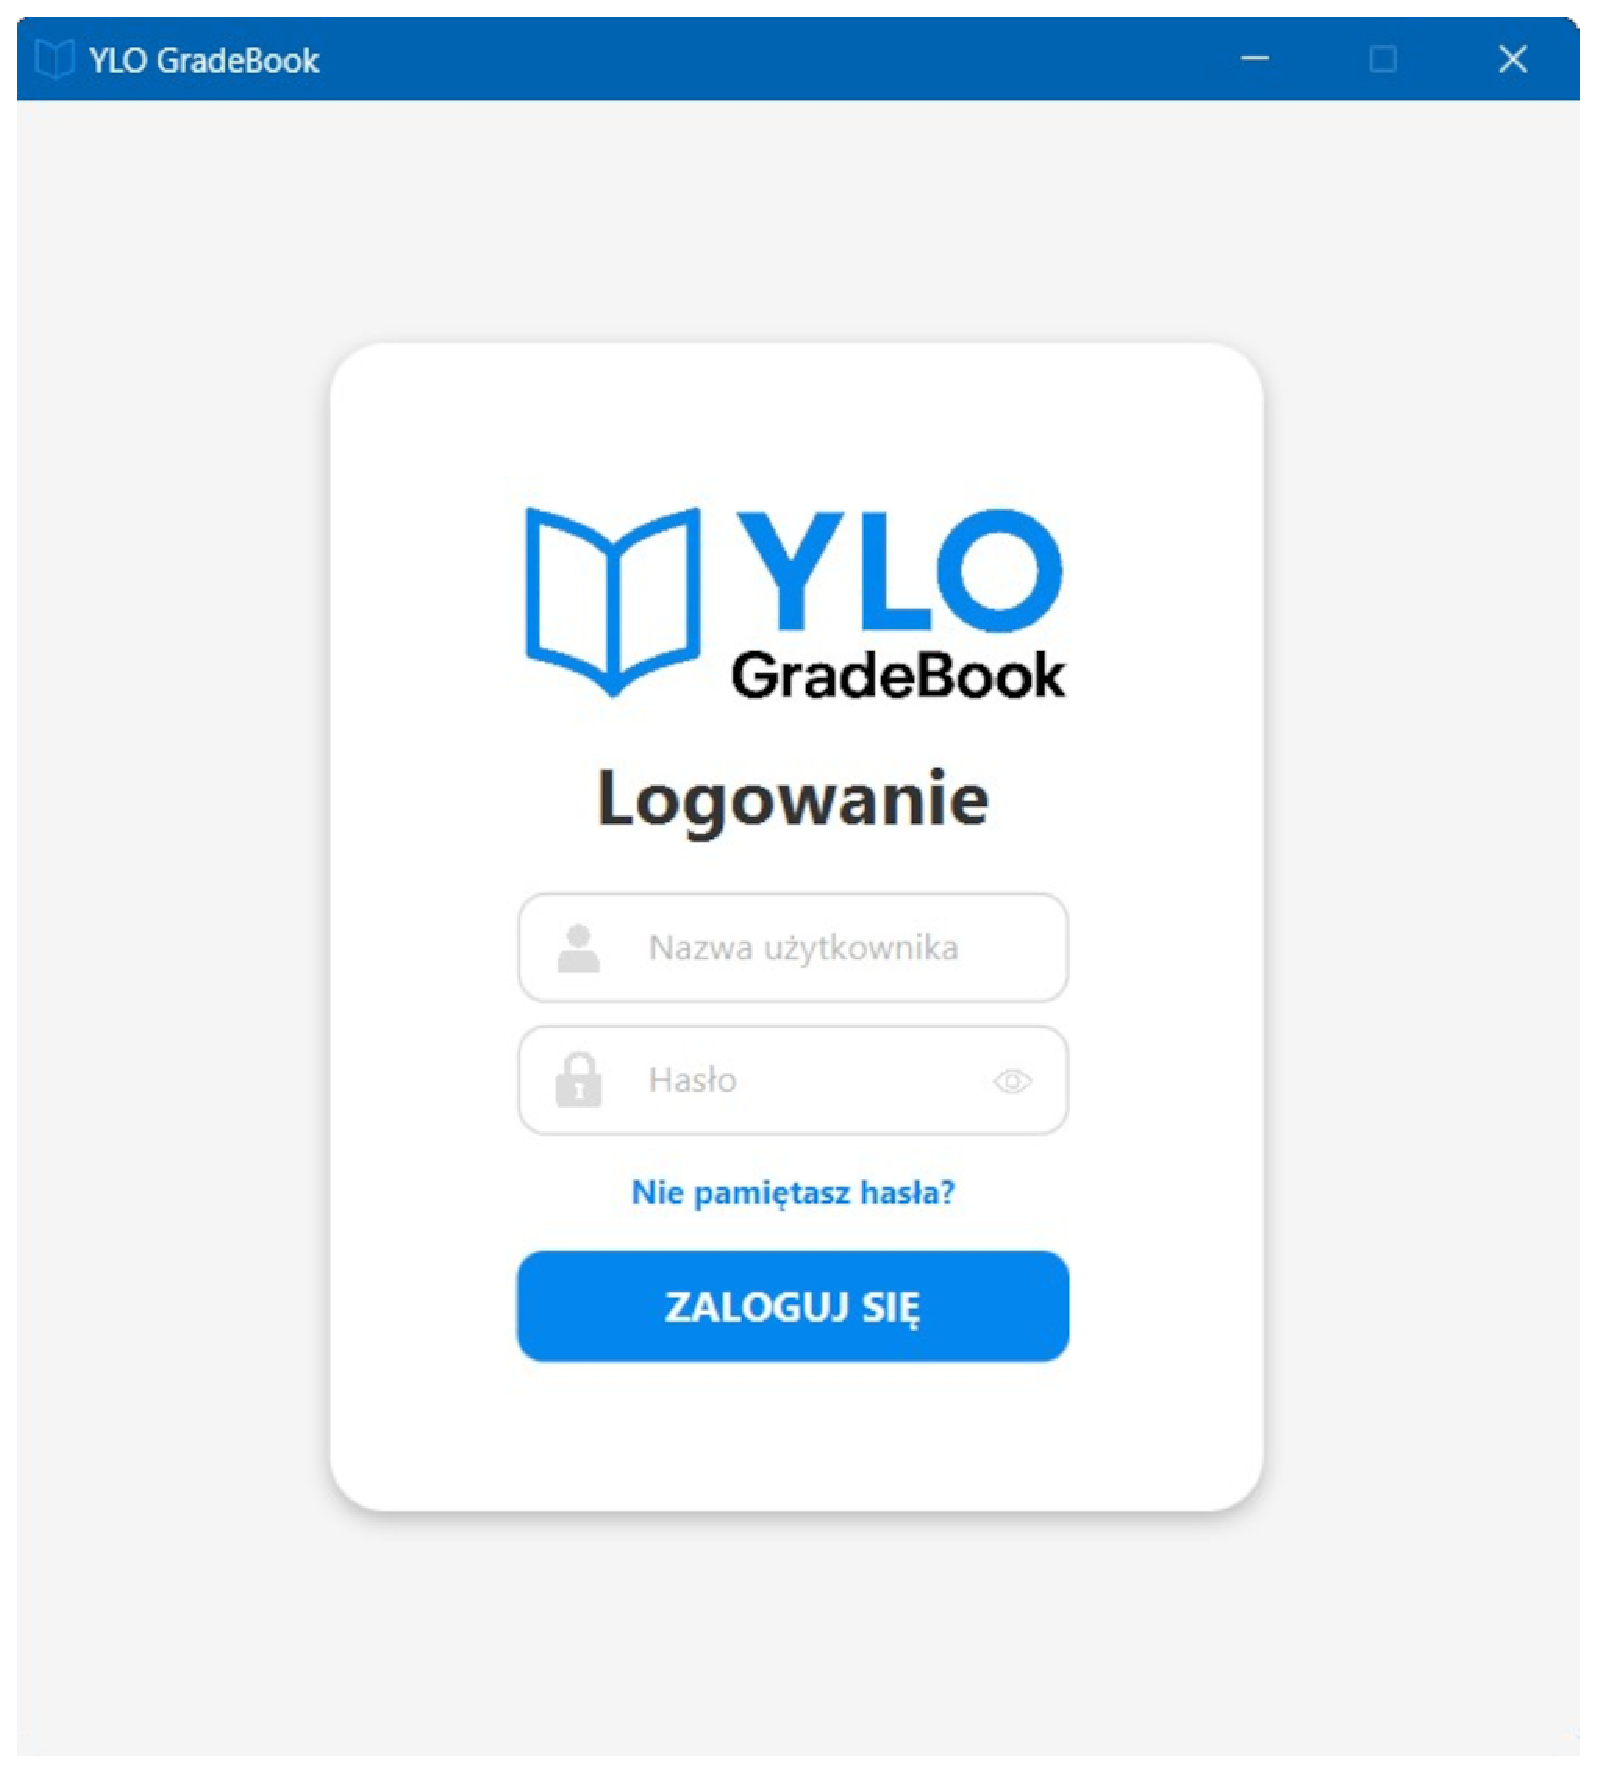
\includegraphics[width=0.9\textwidth]{figures/fig_0005.eps}
    \caption{Okno logowania - weryfikacja danych uwierzytelniających}
    \label{fig:loginView}
\end{figure}
\newpage
\subsection{Okno resetowania hasła}
Widok ten umożliwia zresetowanie hasła użytkownika poprzez podanie jego nazwy konta oraz nowego hasła. Na tym etapie proces nie zawiera jeszcze pełnych mechanizmów bezpieczeństwa (np. weryfikacji mailowej), jednak przewidziano ich wdrożenie w przyszłych wersjach aplikacji.

\begin{itemize}
    \item Interfejs posiada trzy pola: \textbf{Nazwa użytkownika}, \textbf{Hasło} oraz \textbf{Potwierdź hasło}. Posiada również przycisk \textbf{Anuluj} oraz przycisk \textbf{Resetuj hasło}, który pozwala na zaaktualizowanie hasła w bazie danych.
    \item Podobnie jak w przypadku okna logowania dodano możliwość wyświetlenia haseł.
    \item W przypadku błędnego wypełnienia pól pojawia się komunikat.
\end{itemize}

\begin{figure}[H]
    \centering
    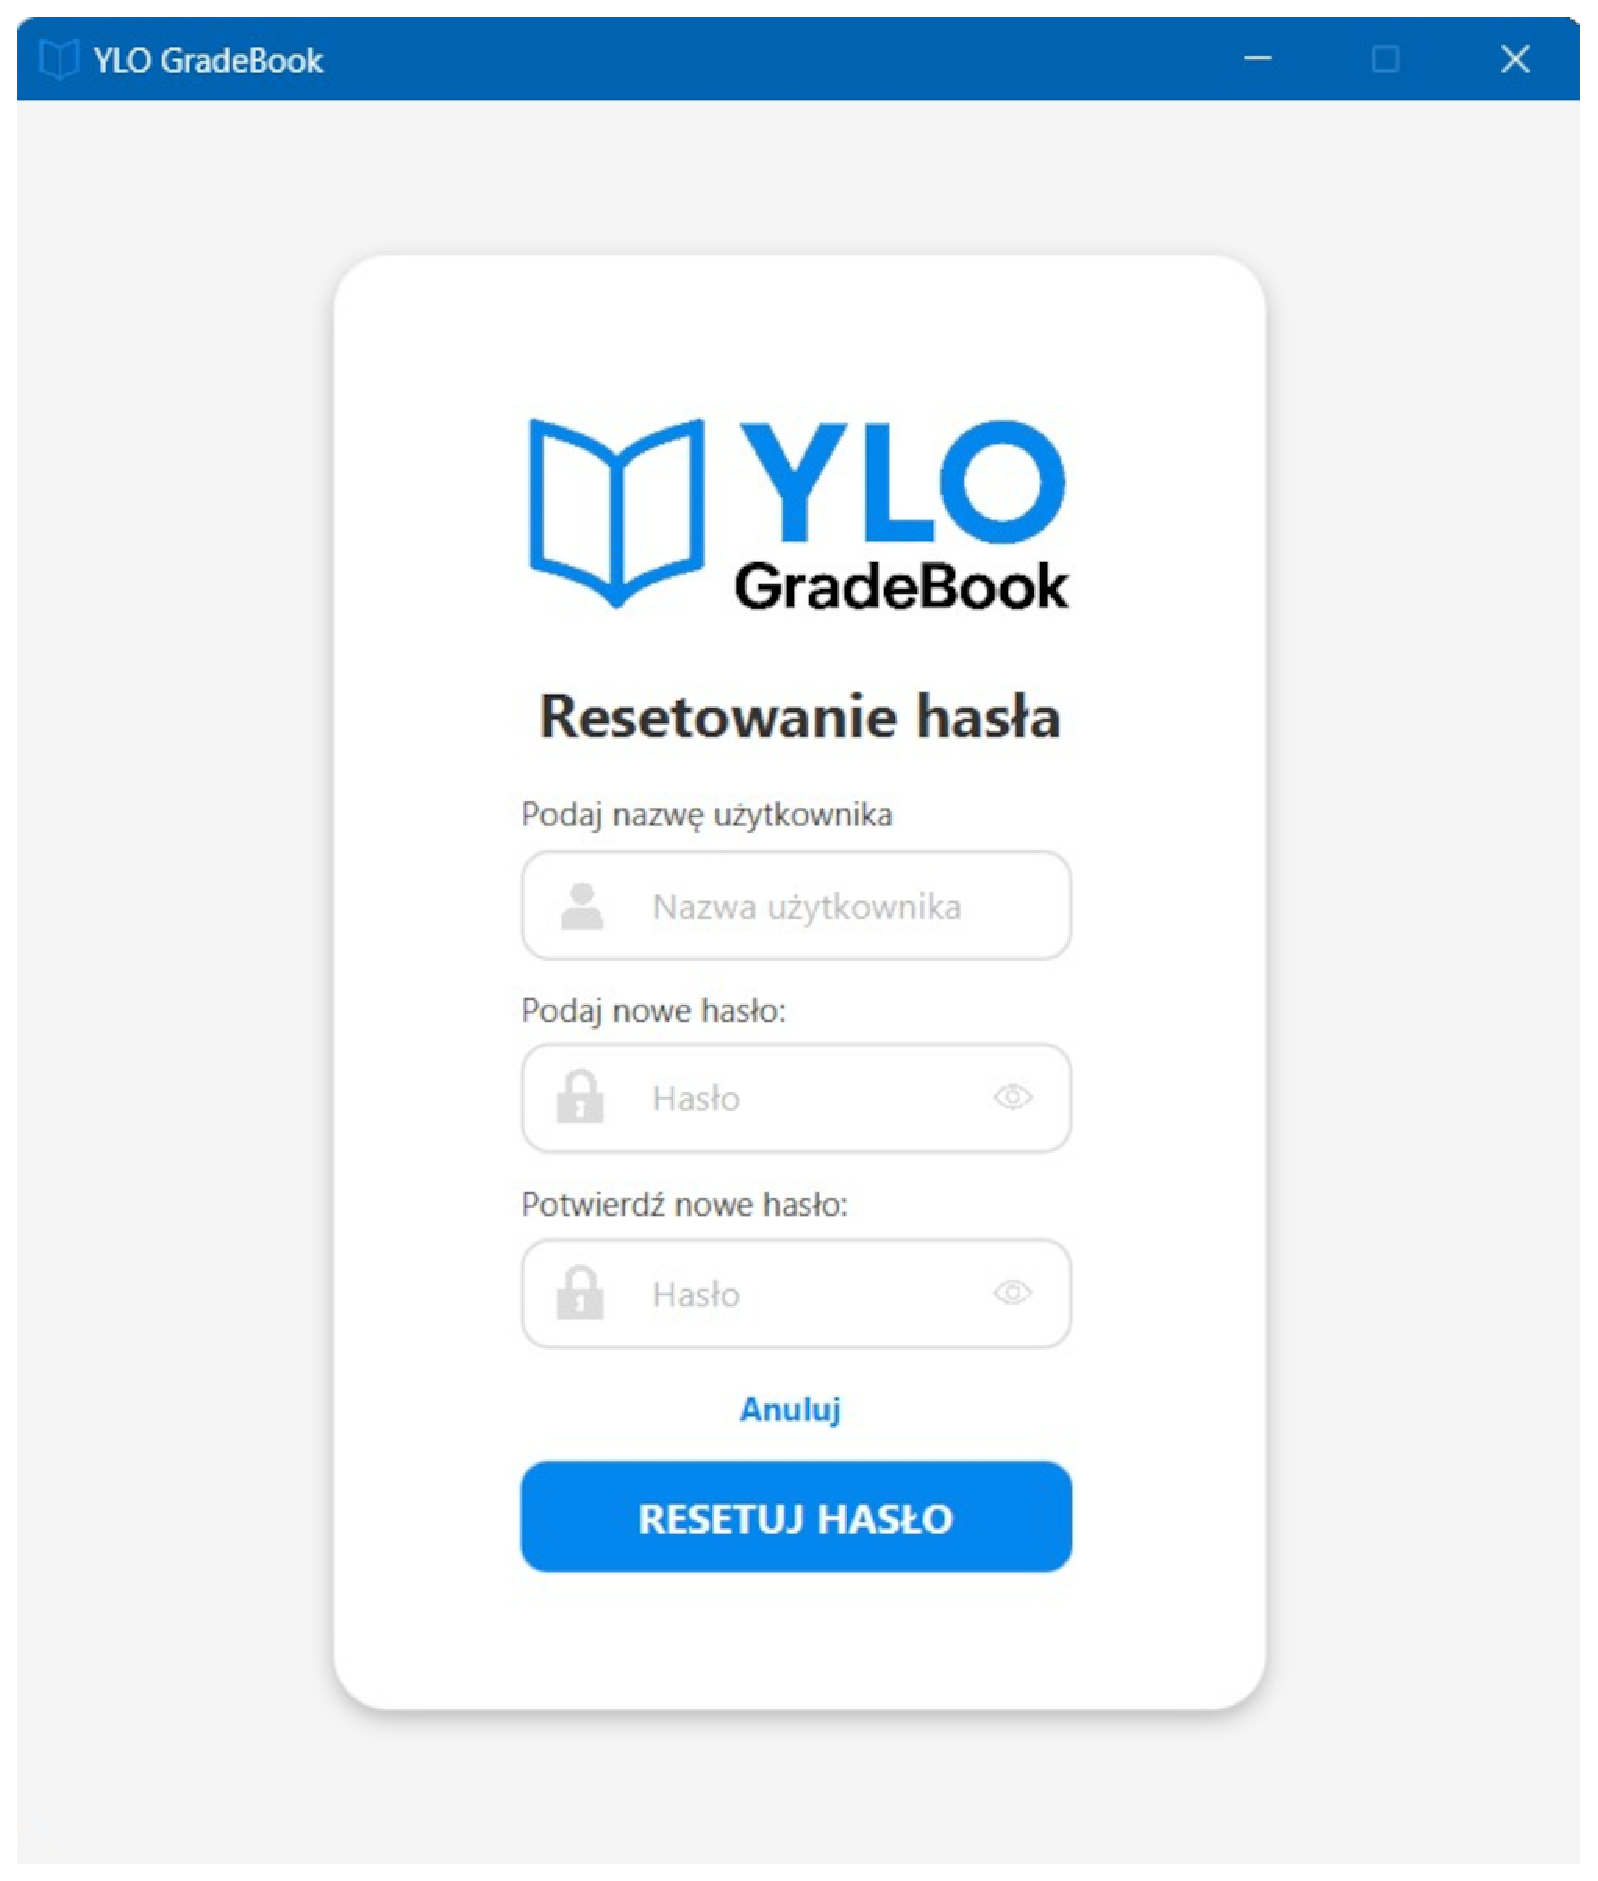
\includegraphics[width=0.9\textwidth]{figures/fig_0006.eps}
    \caption{Okno resetowania hasła - aktualizacja hasła w bazie danych}
    \label{fig:passwordReset}
\end{figure}


\subsection{Główne okno interfejsu ucznia}

Główne okno interfejsu ucznia pojawia się bezpośrednio po jego zalogowaniu do systemu \texttt{YLO GradeBook}. Zostało zaprojektowane z myślą o szybkim i intuicyjnym dostępie do najważniejszych informacji oraz funkcji systemu. Podział treści na zakładki oraz wyraźna struktura ułatwiają poruszanie się po aplikacji.

\begin{itemize}
    \item Po lewej stronie znajduje się panel nawigacyjny z zakładkami: \textbf{Strona główna}, \textbf{Oceny}, \textbf{Terminarz}, \textbf{Uwagi}, \textbf{Notatki}, \textbf{Konto} oraz \textbf{Ustawienia}.
    \item W górnej części widoku wyświetlane jest powitanie użytkownika wraz z jego imieniem, a także powiadomienie z liczbą nowych ocen i nadchodzących terminów. Po prawej stronie znajduje się przycisk \textbf{Wyloguj}, umożliwiający zakończenie sesji.
    \item Centralną część okna zajmuje sekcja \textbf{Najnowsze oceny}, prezentująca ostatnio dodane wyniki ucznia.
    \item Po prawej stronie umieszczono szybkie odnośniki do najczęściej wykorzystywanych zakładek, co ułatwia nawigację. W tym miejscu znajduje się również panel ze średnią, który po kliknięciu ukazuje ogólną średnią ucznia.
\end{itemize}

Taki układ pozwala użytkownikowi w intuicyjny sposób monitorować postępy oraz mieć wgląd w najnowsze wydarzenia.

\begin{figure}[H]
    \centering
    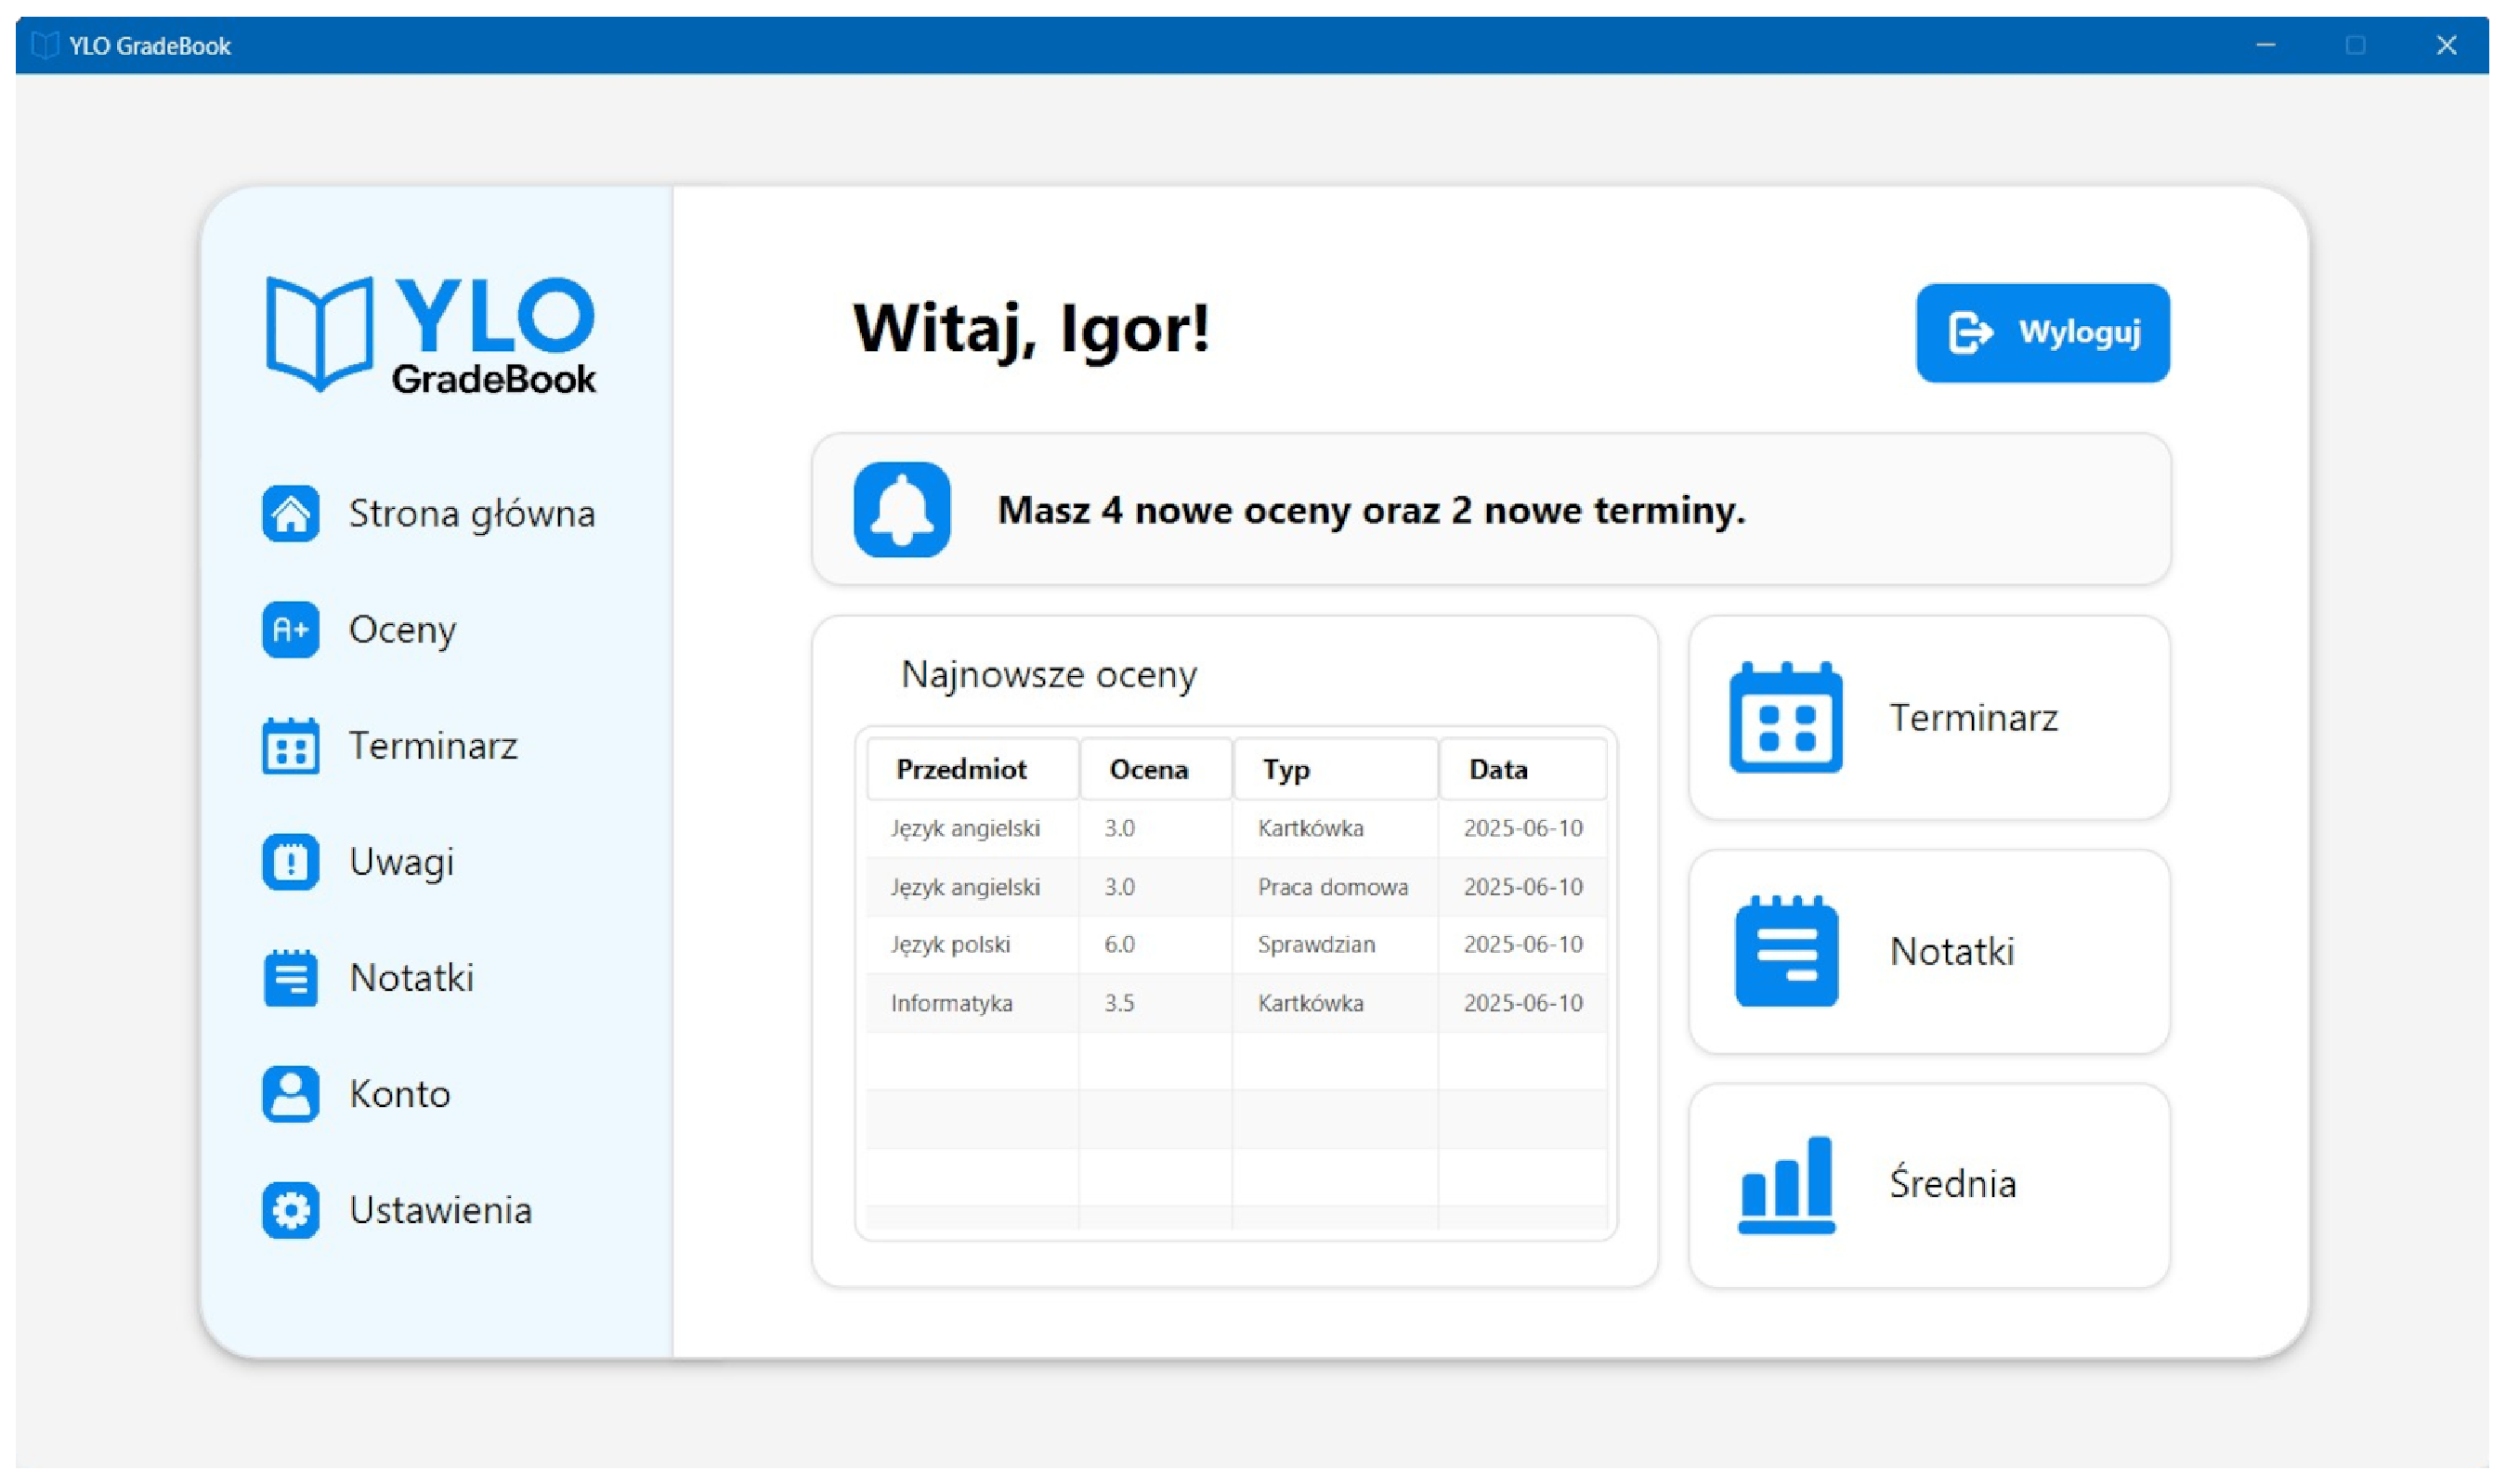
\includegraphics[width=0.9\textwidth]{figures/fig_0007.eps}
    \caption{Główny widok ucznia}
    \label{fig:studentWindow}
\end{figure}
\newpage
\subsubsection{Zakładka „Oceny”}
Widok ten umożliwia uczniowi przegląd ocen z podziałem na przedmioty oraz wyświetlenie średniej ocen z każdego z nich.
\begin{figure}[H]
    \centering
    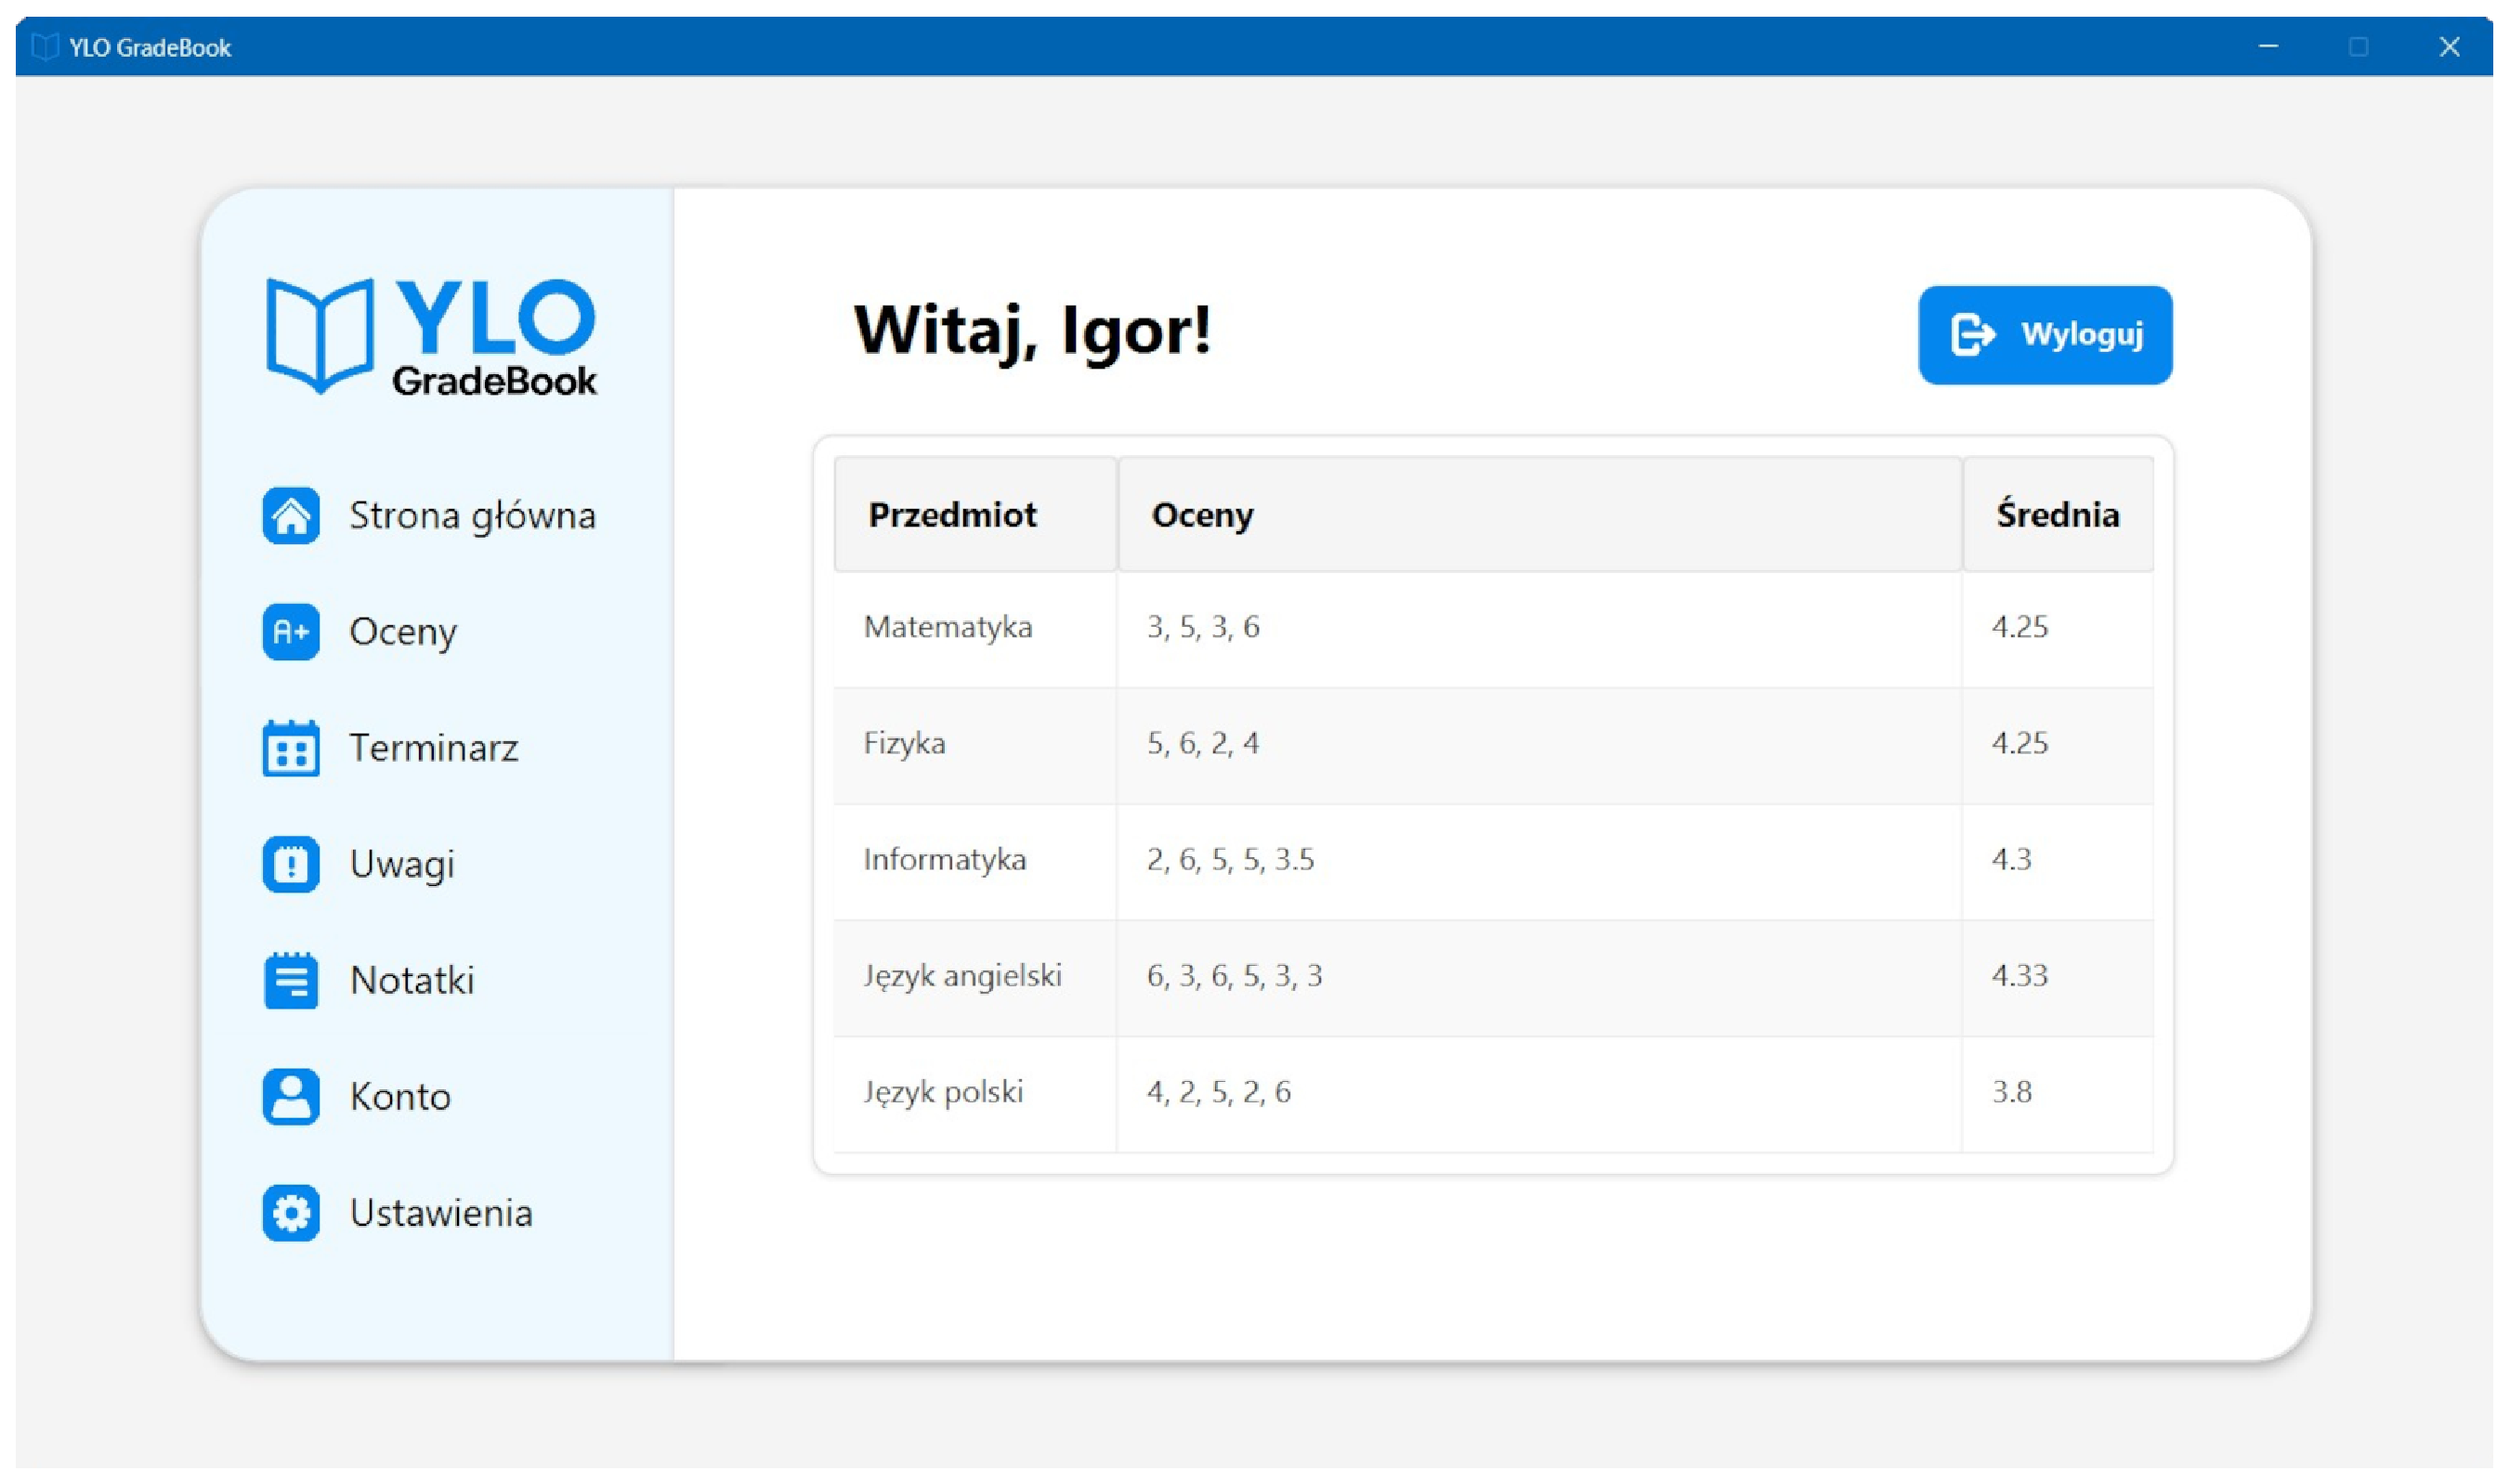
\includegraphics[width=0.9\textwidth]{figures/StudentWindow/fig_0009.eps}
    \caption{Okno ucznia - Zakładka „Oceny”}
    \label{fig:studentGradePane}
\end{figure}

\subsubsection{Zakładka „Terminarz”}
Zakładka służy do wyświetlania wszystkich nadchodzących terminów wydarzeń przypisanych do klasy ucznia.
\begin{figure}[H]
    \centering
    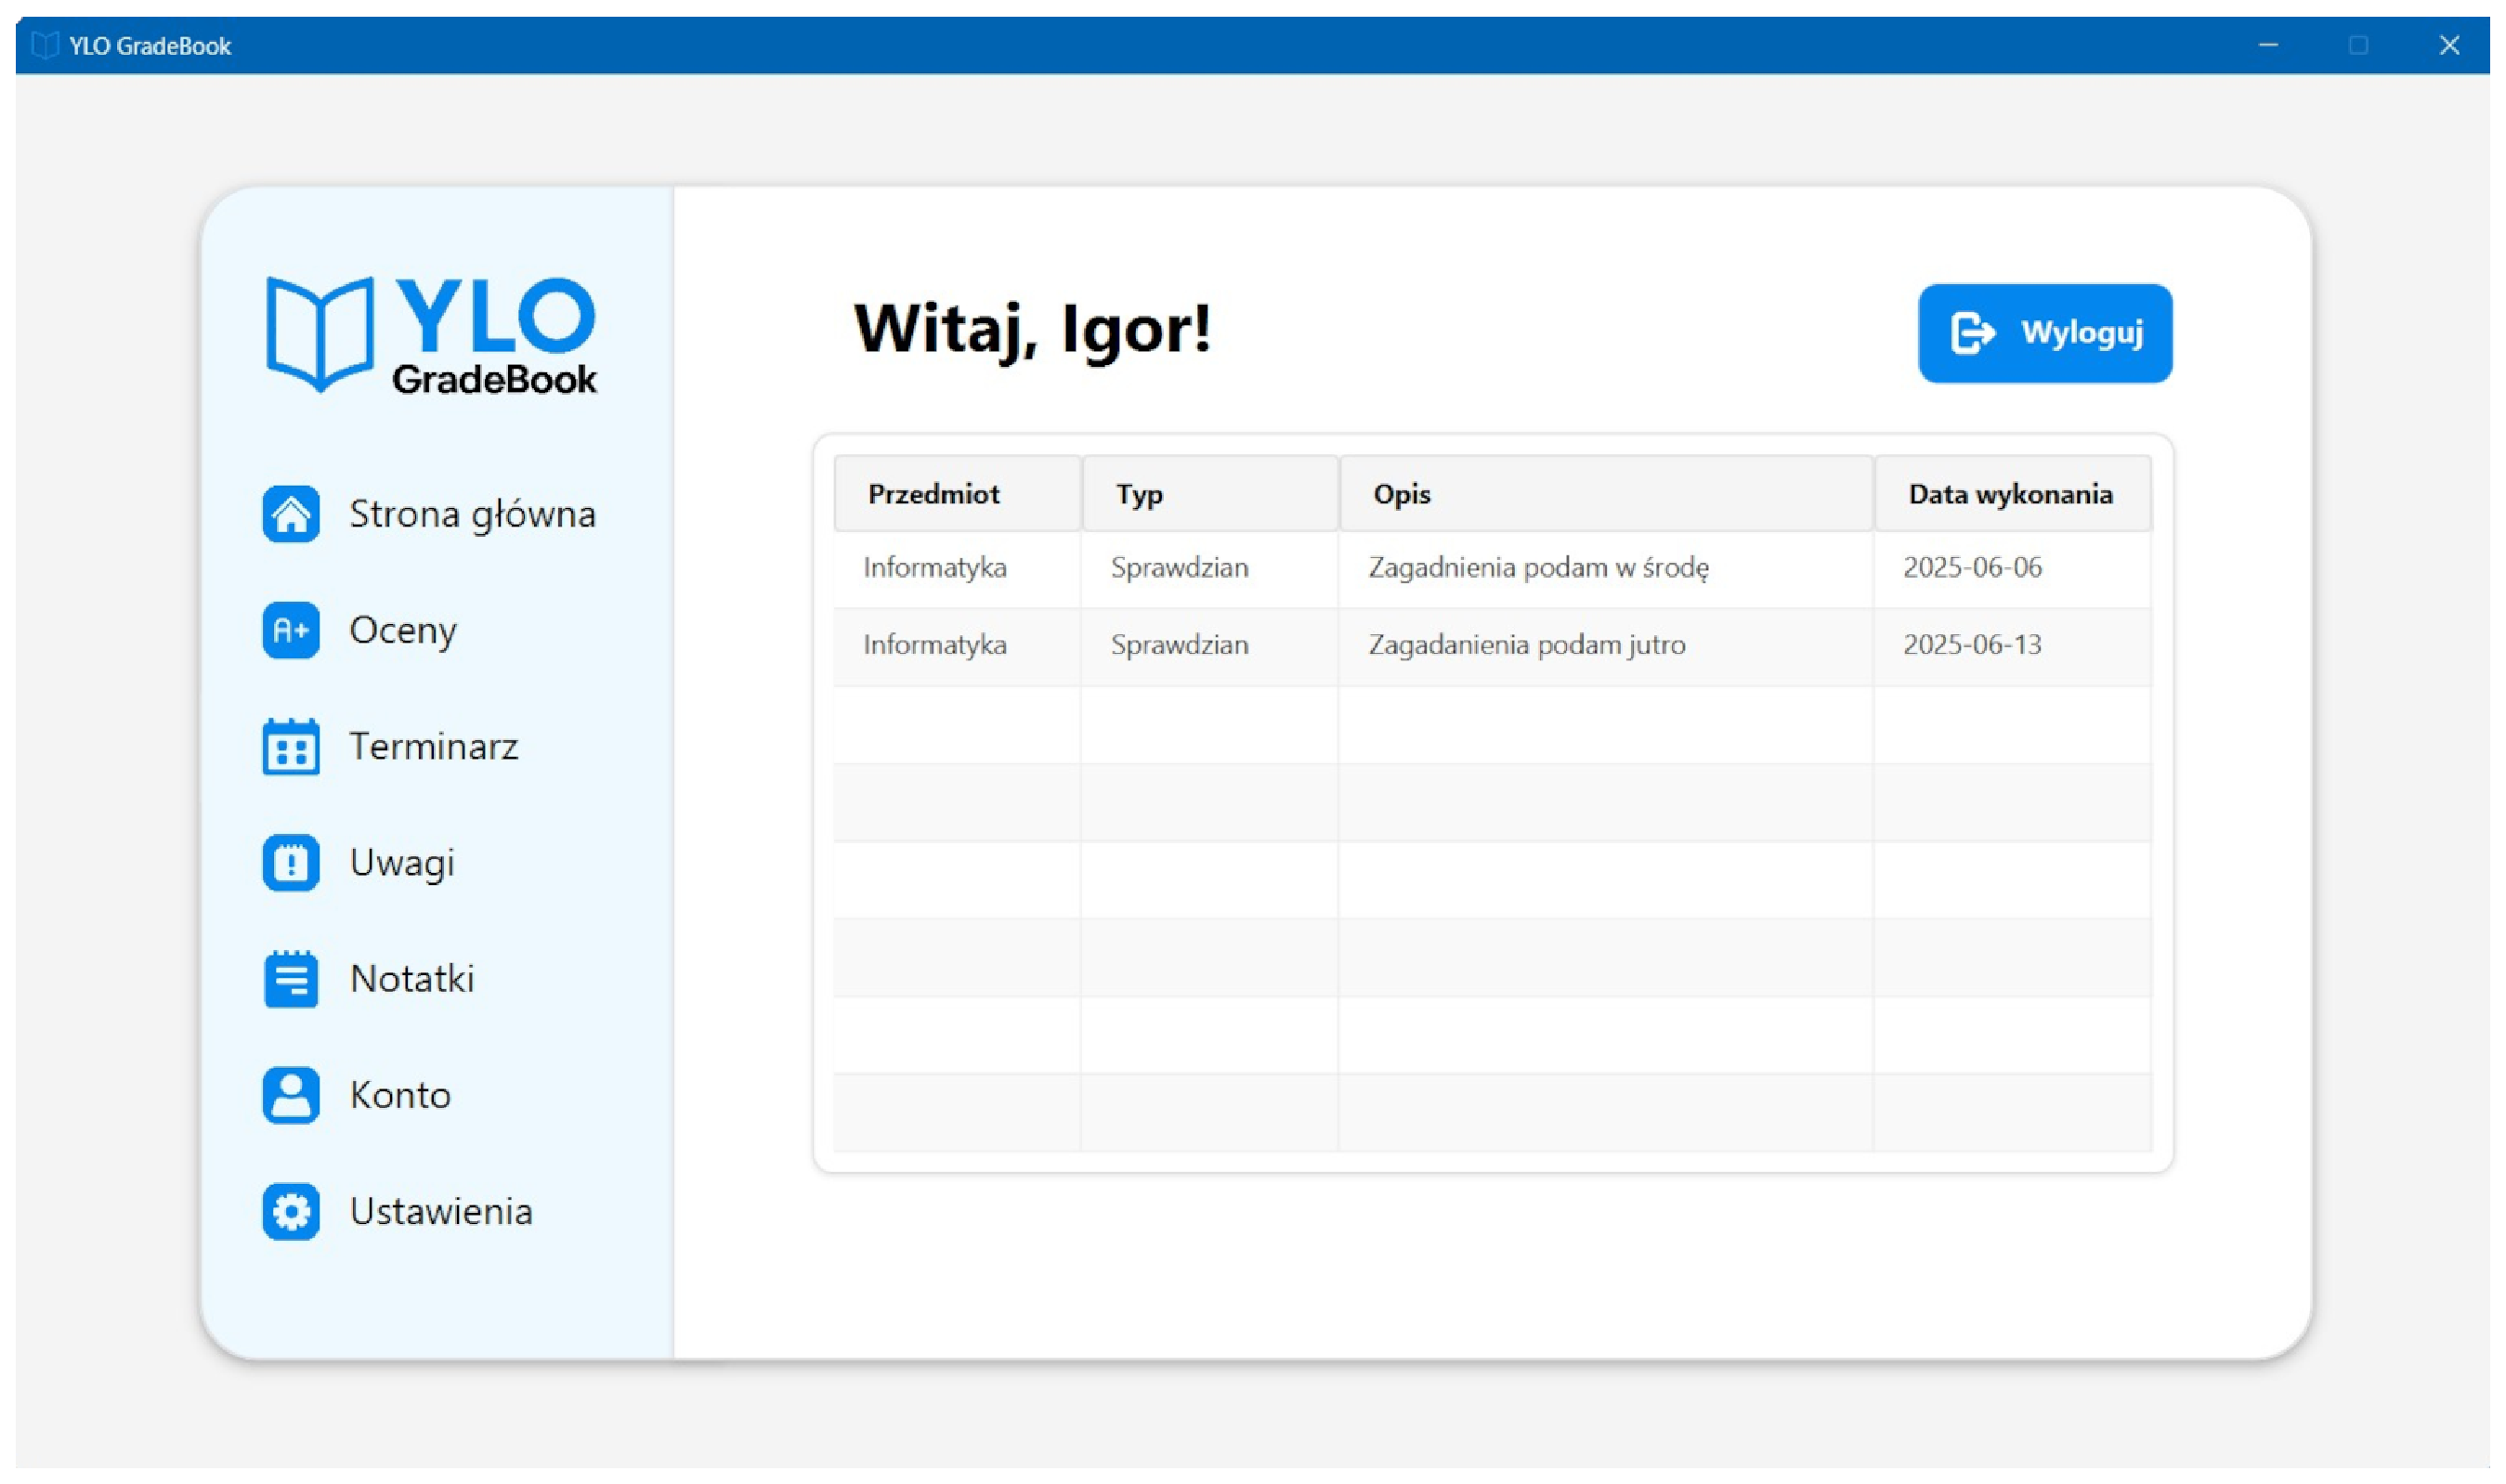
\includegraphics[width=0.9\textwidth]{figures/StudentWindow/fig_0010.eps}
    \caption{Okno ucznia - Zakładka „Terminarz”}
    \label{fig:studentDaedLinePane}
\end{figure}
\newpage
\subsubsection{Zakładka „Uwagi”}
Zakładka umożliwia przegląd uwag przypisanych do konta ucznia.
\begin{figure}[H]
    \centering
    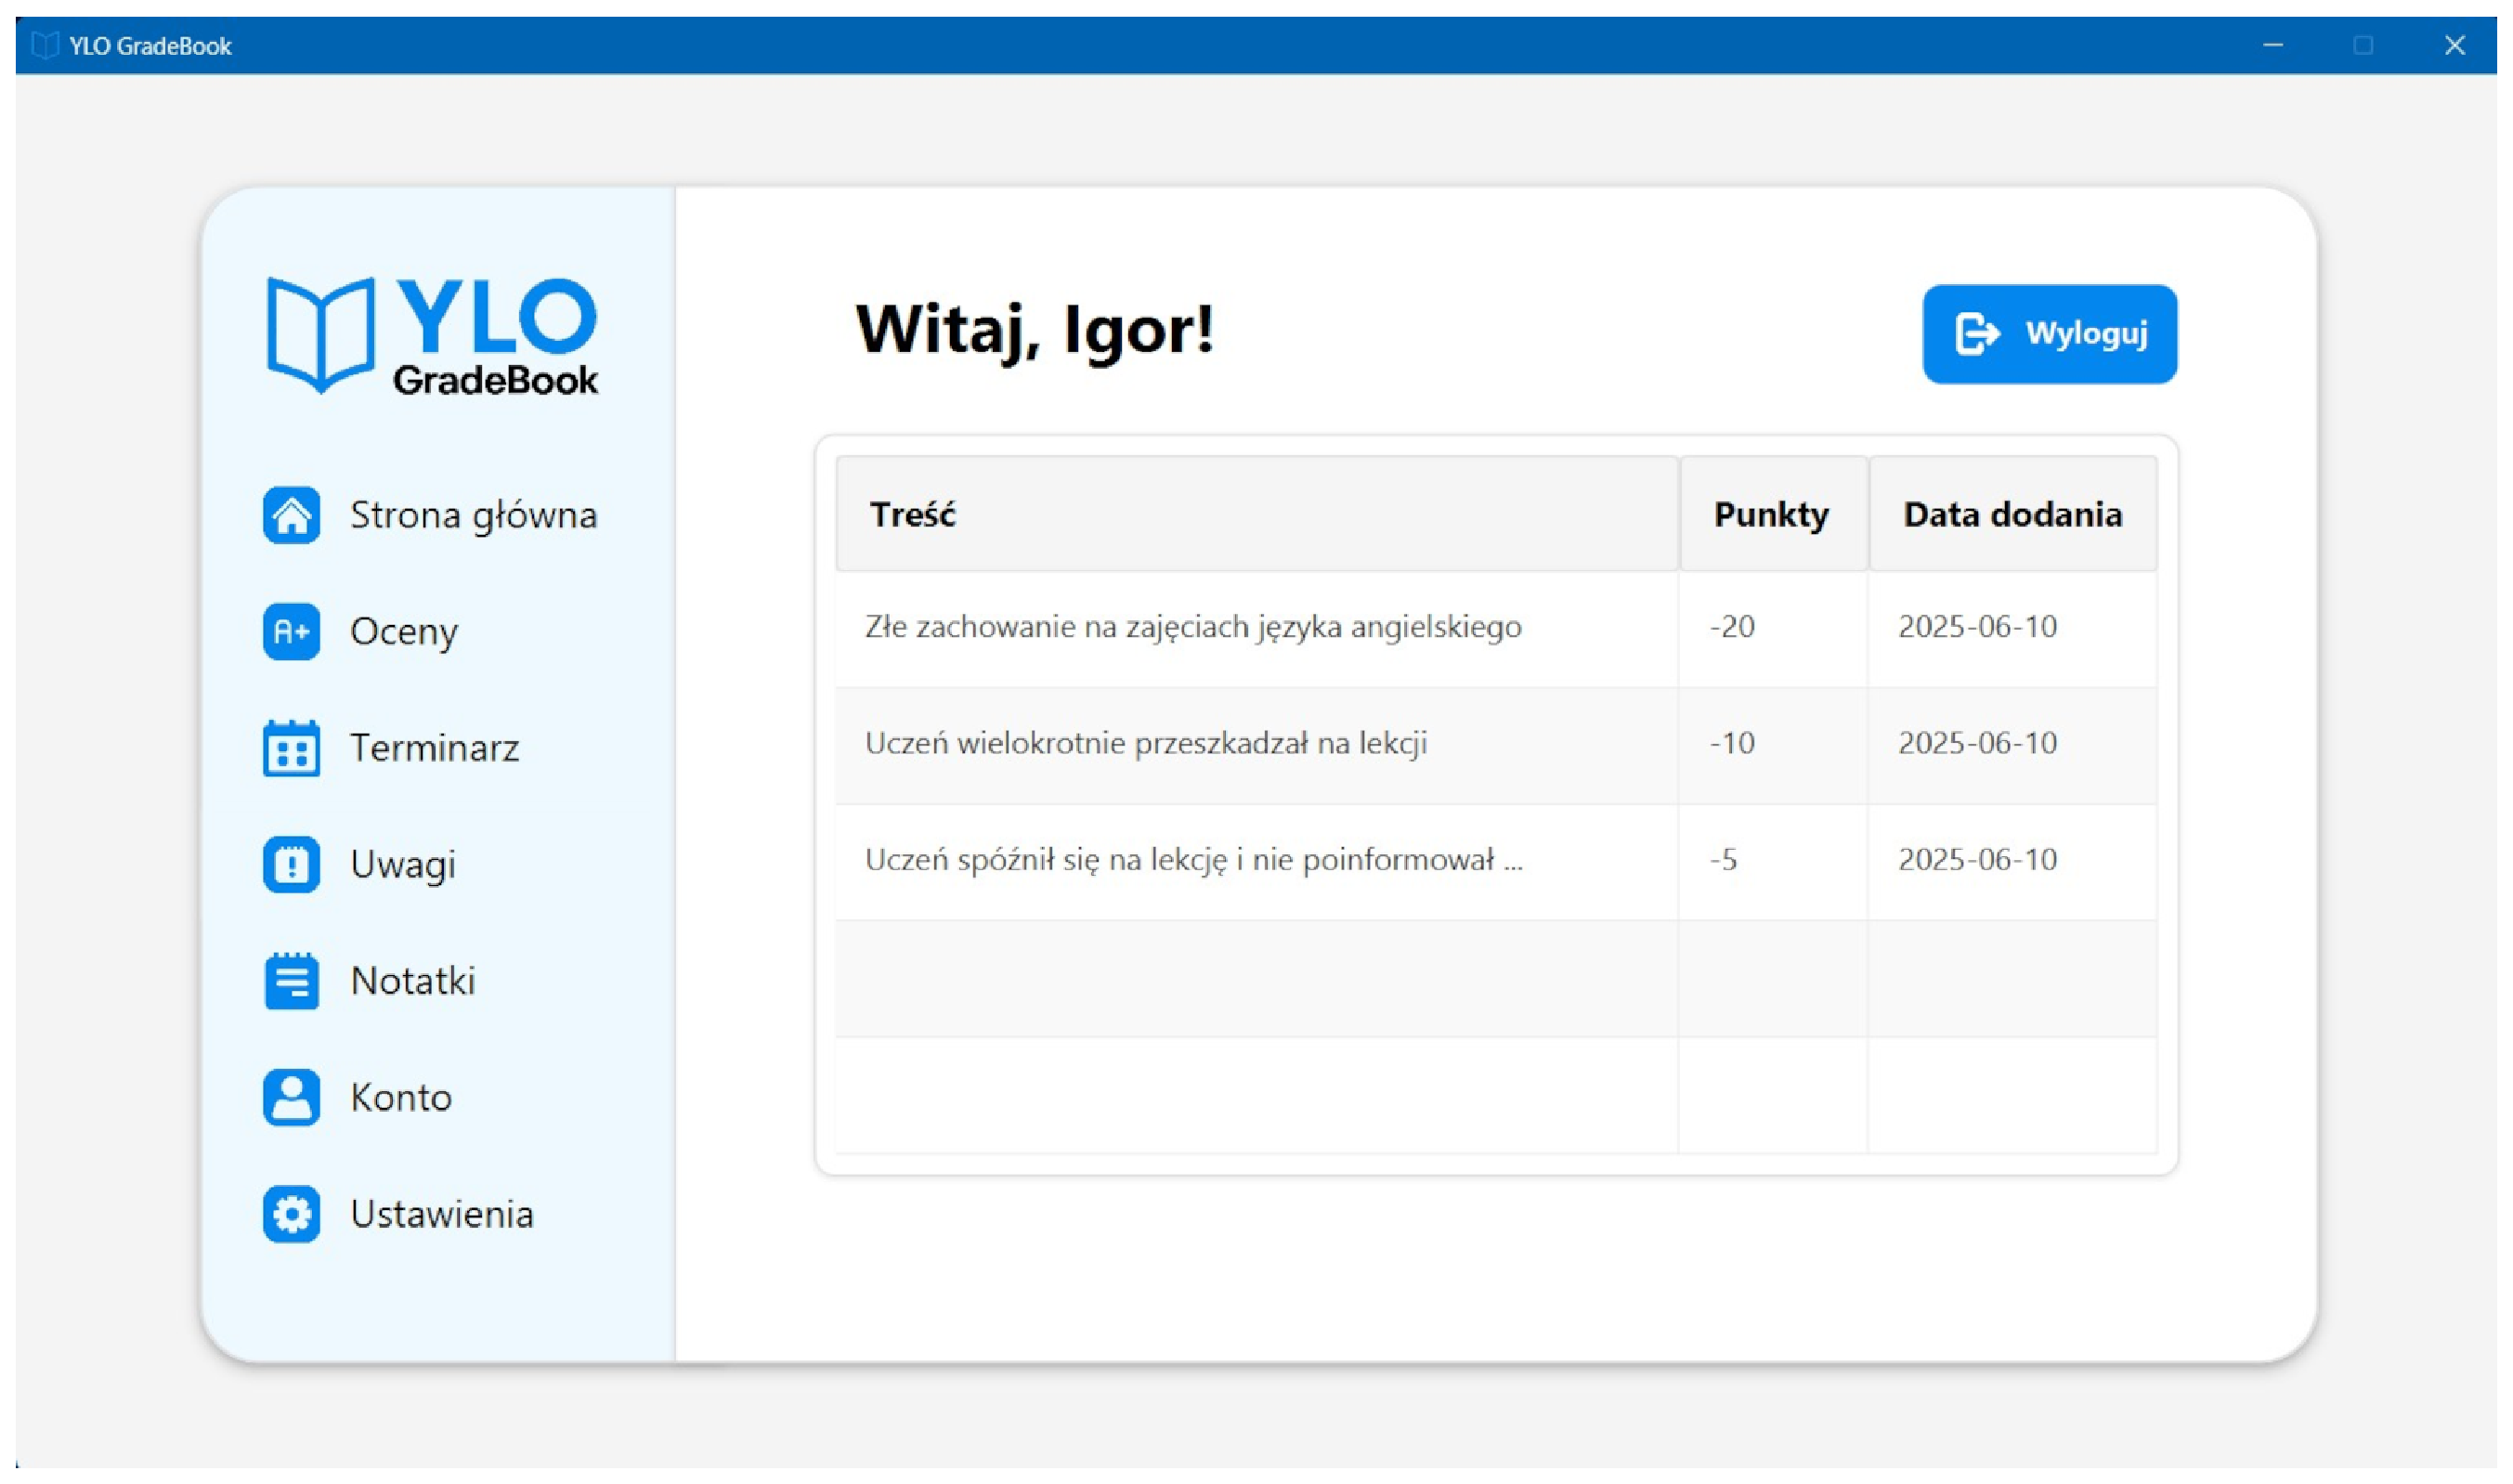
\includegraphics[width=0.9\textwidth]{figures/StudentWindow/fig_0011.eps}
    \caption{Okno ucznia - Zakładka „Uwagi”}
    \label{fig:studentNegativeNotesPane}
\end{figure}

\subsection*{Pozostałe zakładki}
Pozostałe zakładki zostaną zaprezentowane zbiorczo na końcu podrozdziału, ponieważ ich wygląd i funkcjonalność są identyczne niezależnie od przypisanej roli użytkownika
\newpage
\subsection{Główne okno interfejsu nauczyciela}
Główne okno interfejsu nauczyciela pojawia się bezpośrednio po jego zalogowaniu do systemu \texttt{YLO GradeBook}. Zostało zaprojektowane z myślą o szybkim i intuicyjnym dostępie do najważniejszych funkcji systemu. Podział treści na zakładki oraz wyraźna struktura interfejsu ułatwiają sprawne poruszanie się po aplikacji.
\begin{itemize}
    \item Po lewej stronie znajduje się panel nawigacyjny z zakładkami: \textbf{Strona główna}, \textbf{Oceny}, \textbf{Notatki}, \textbf{Konto} oraz \textbf{Ustawienia}.
    \item W górnej części widoku wyświetlane jest powitanie użytkownika wraz z jego imieniem, a także przycisk odpowiedzialny za kluczową funkcję — \textbf{dodawanie ocen}.
    \item Po prawej stronie umieszczono przycisk \textbf{Wyloguj}, umożliwiający szybkie zakończenie sesji.
    \item Centralna część okna prezentuje listę uczniów aktualnie wybranej klasy.
    \item Po prawej stronie znajdują się szybkie odnośniki do najczęściej wykonywanych operacji.
\end{itemize}

\begin{figure}[H]
    \centering
    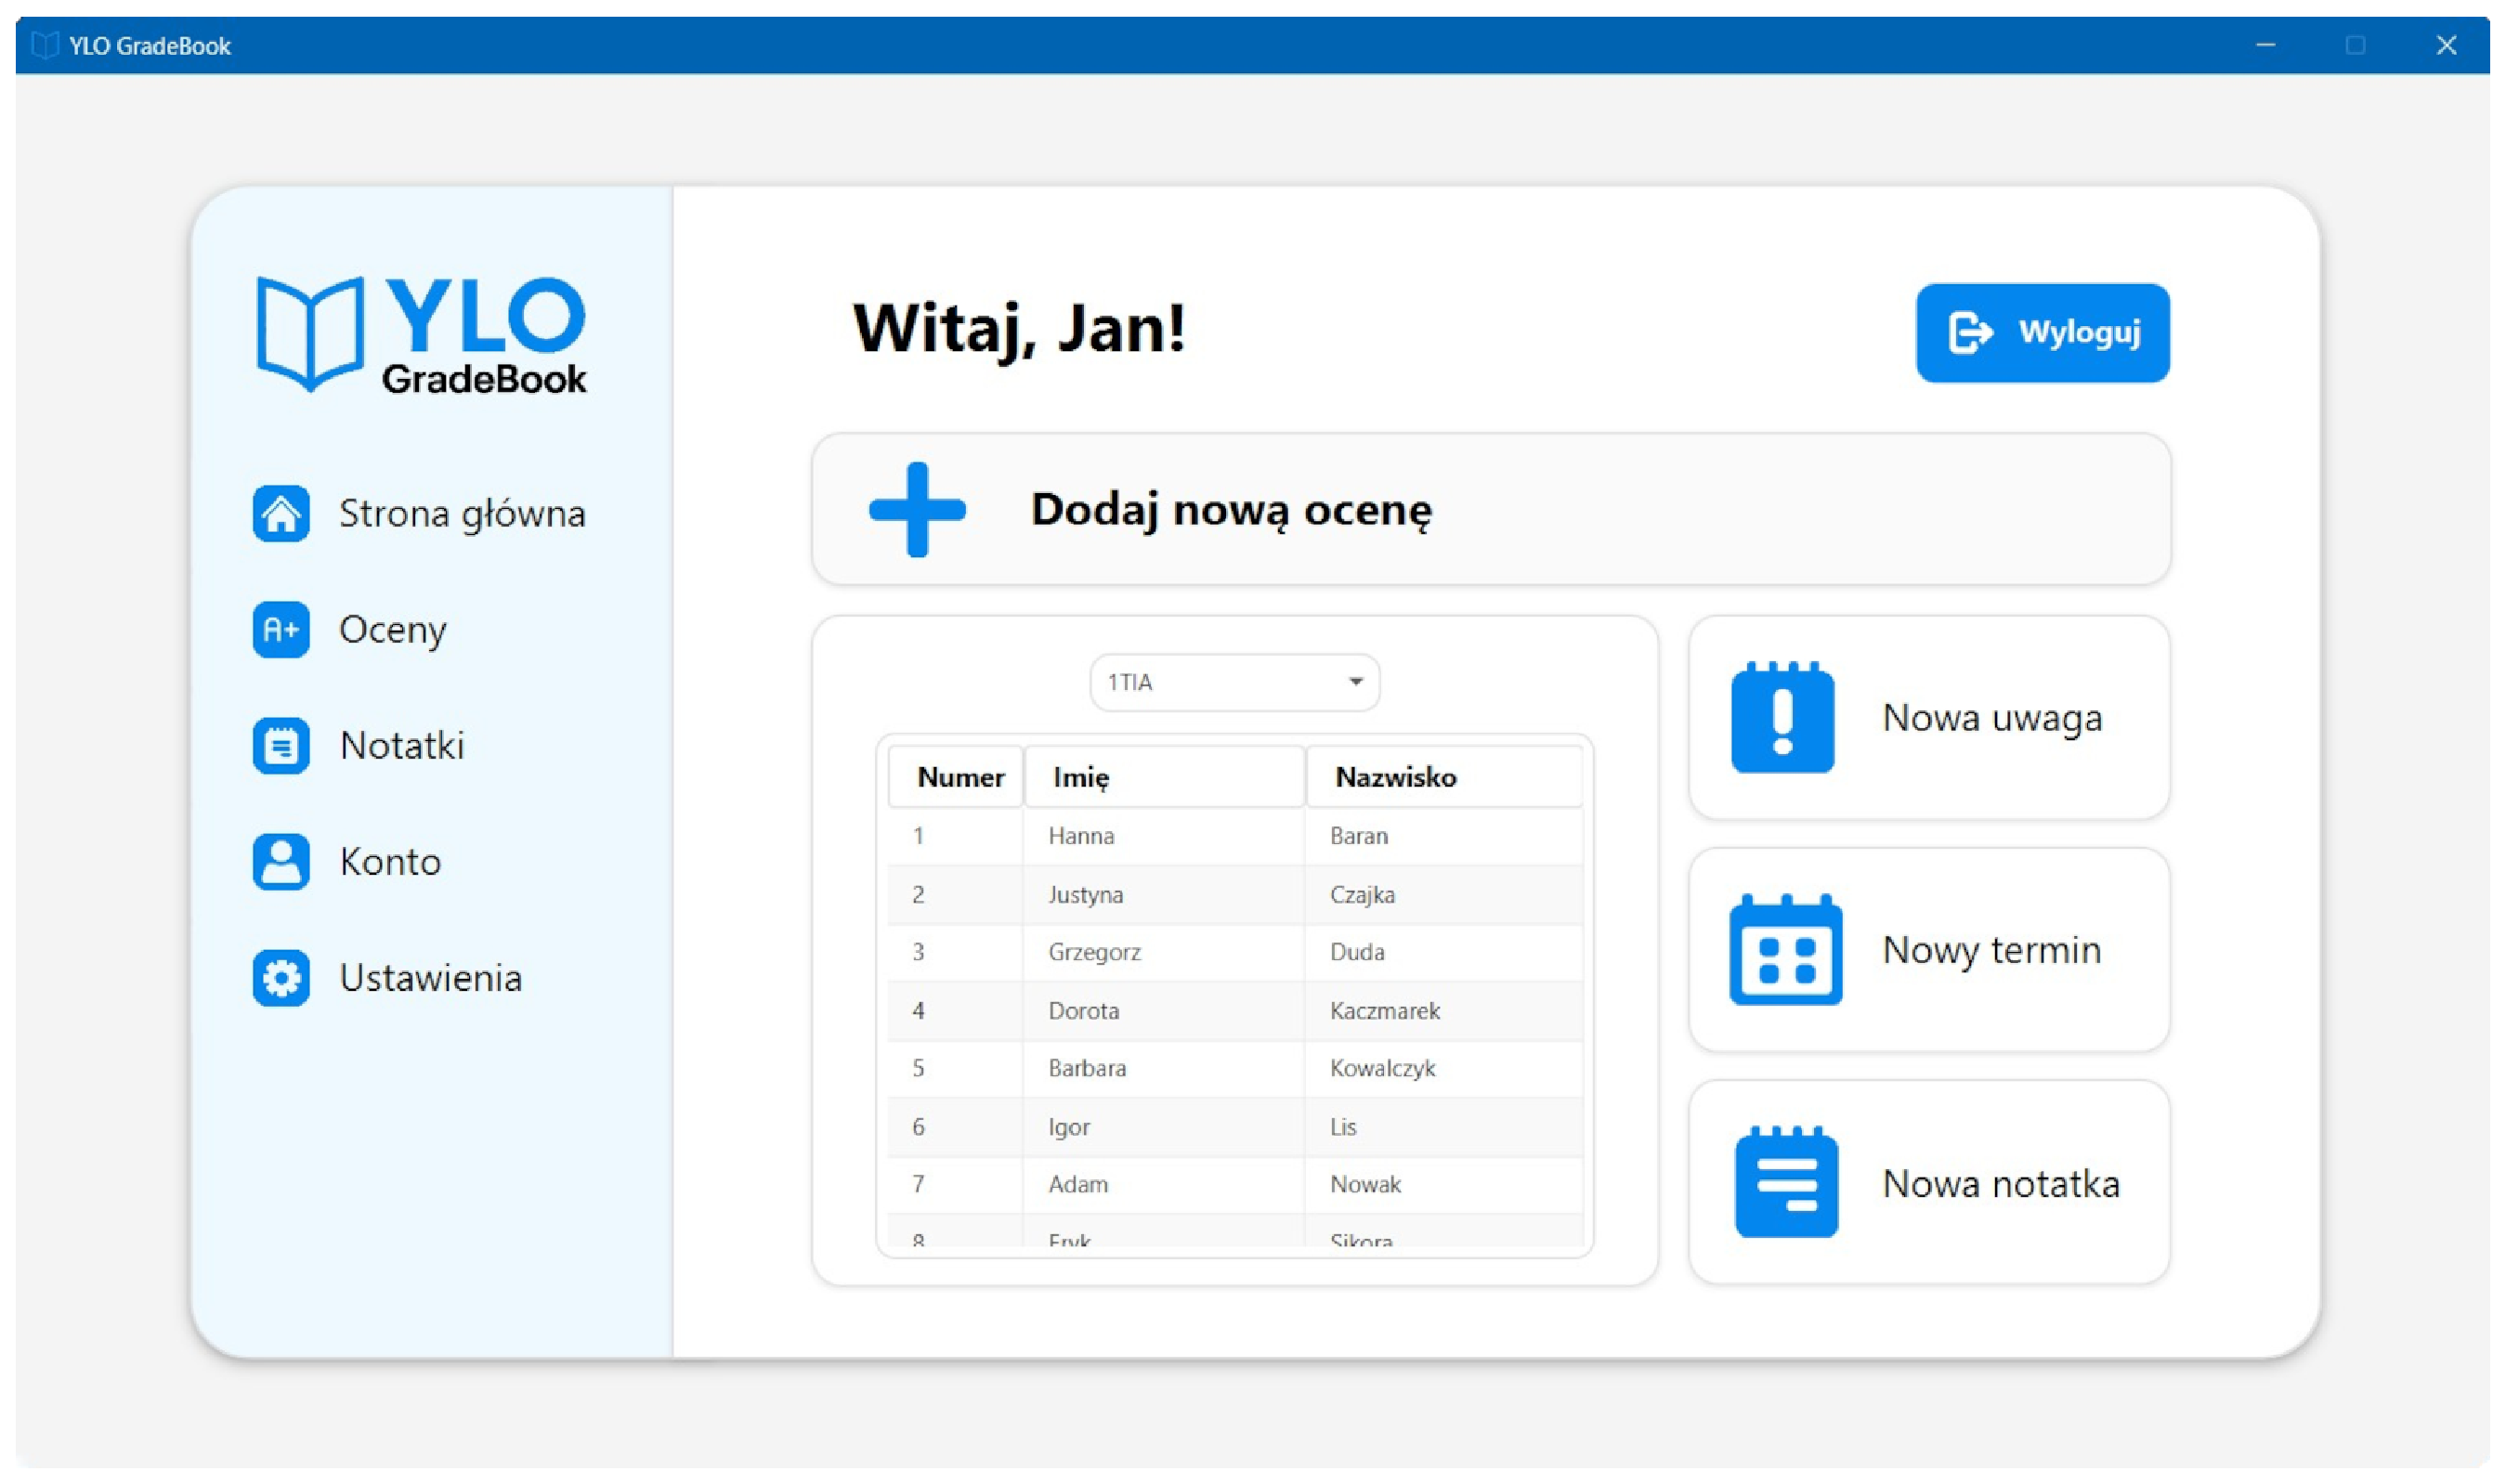
\includegraphics[width=0.9\textwidth]{figures/fig_0008.eps}
    \caption{Główny widok nauczyciela}
    \label{fig:teacherWindow}
\end{figure}
\newpage
\subsubsection{Zakładka „Oceny”}
Zakładka zawiera wyróżniony przycisk umożliwiający otwarcie okna typu pop-up, w którym nauczyciel może przypisać ocenę konkretnemu uczniowi.
Poniżej znajduje się tabela przedstawiająca oceny wszystkich uczniów wybranej klasy z danego przedmiotu.
\begin{figure}[H]
    \centering
    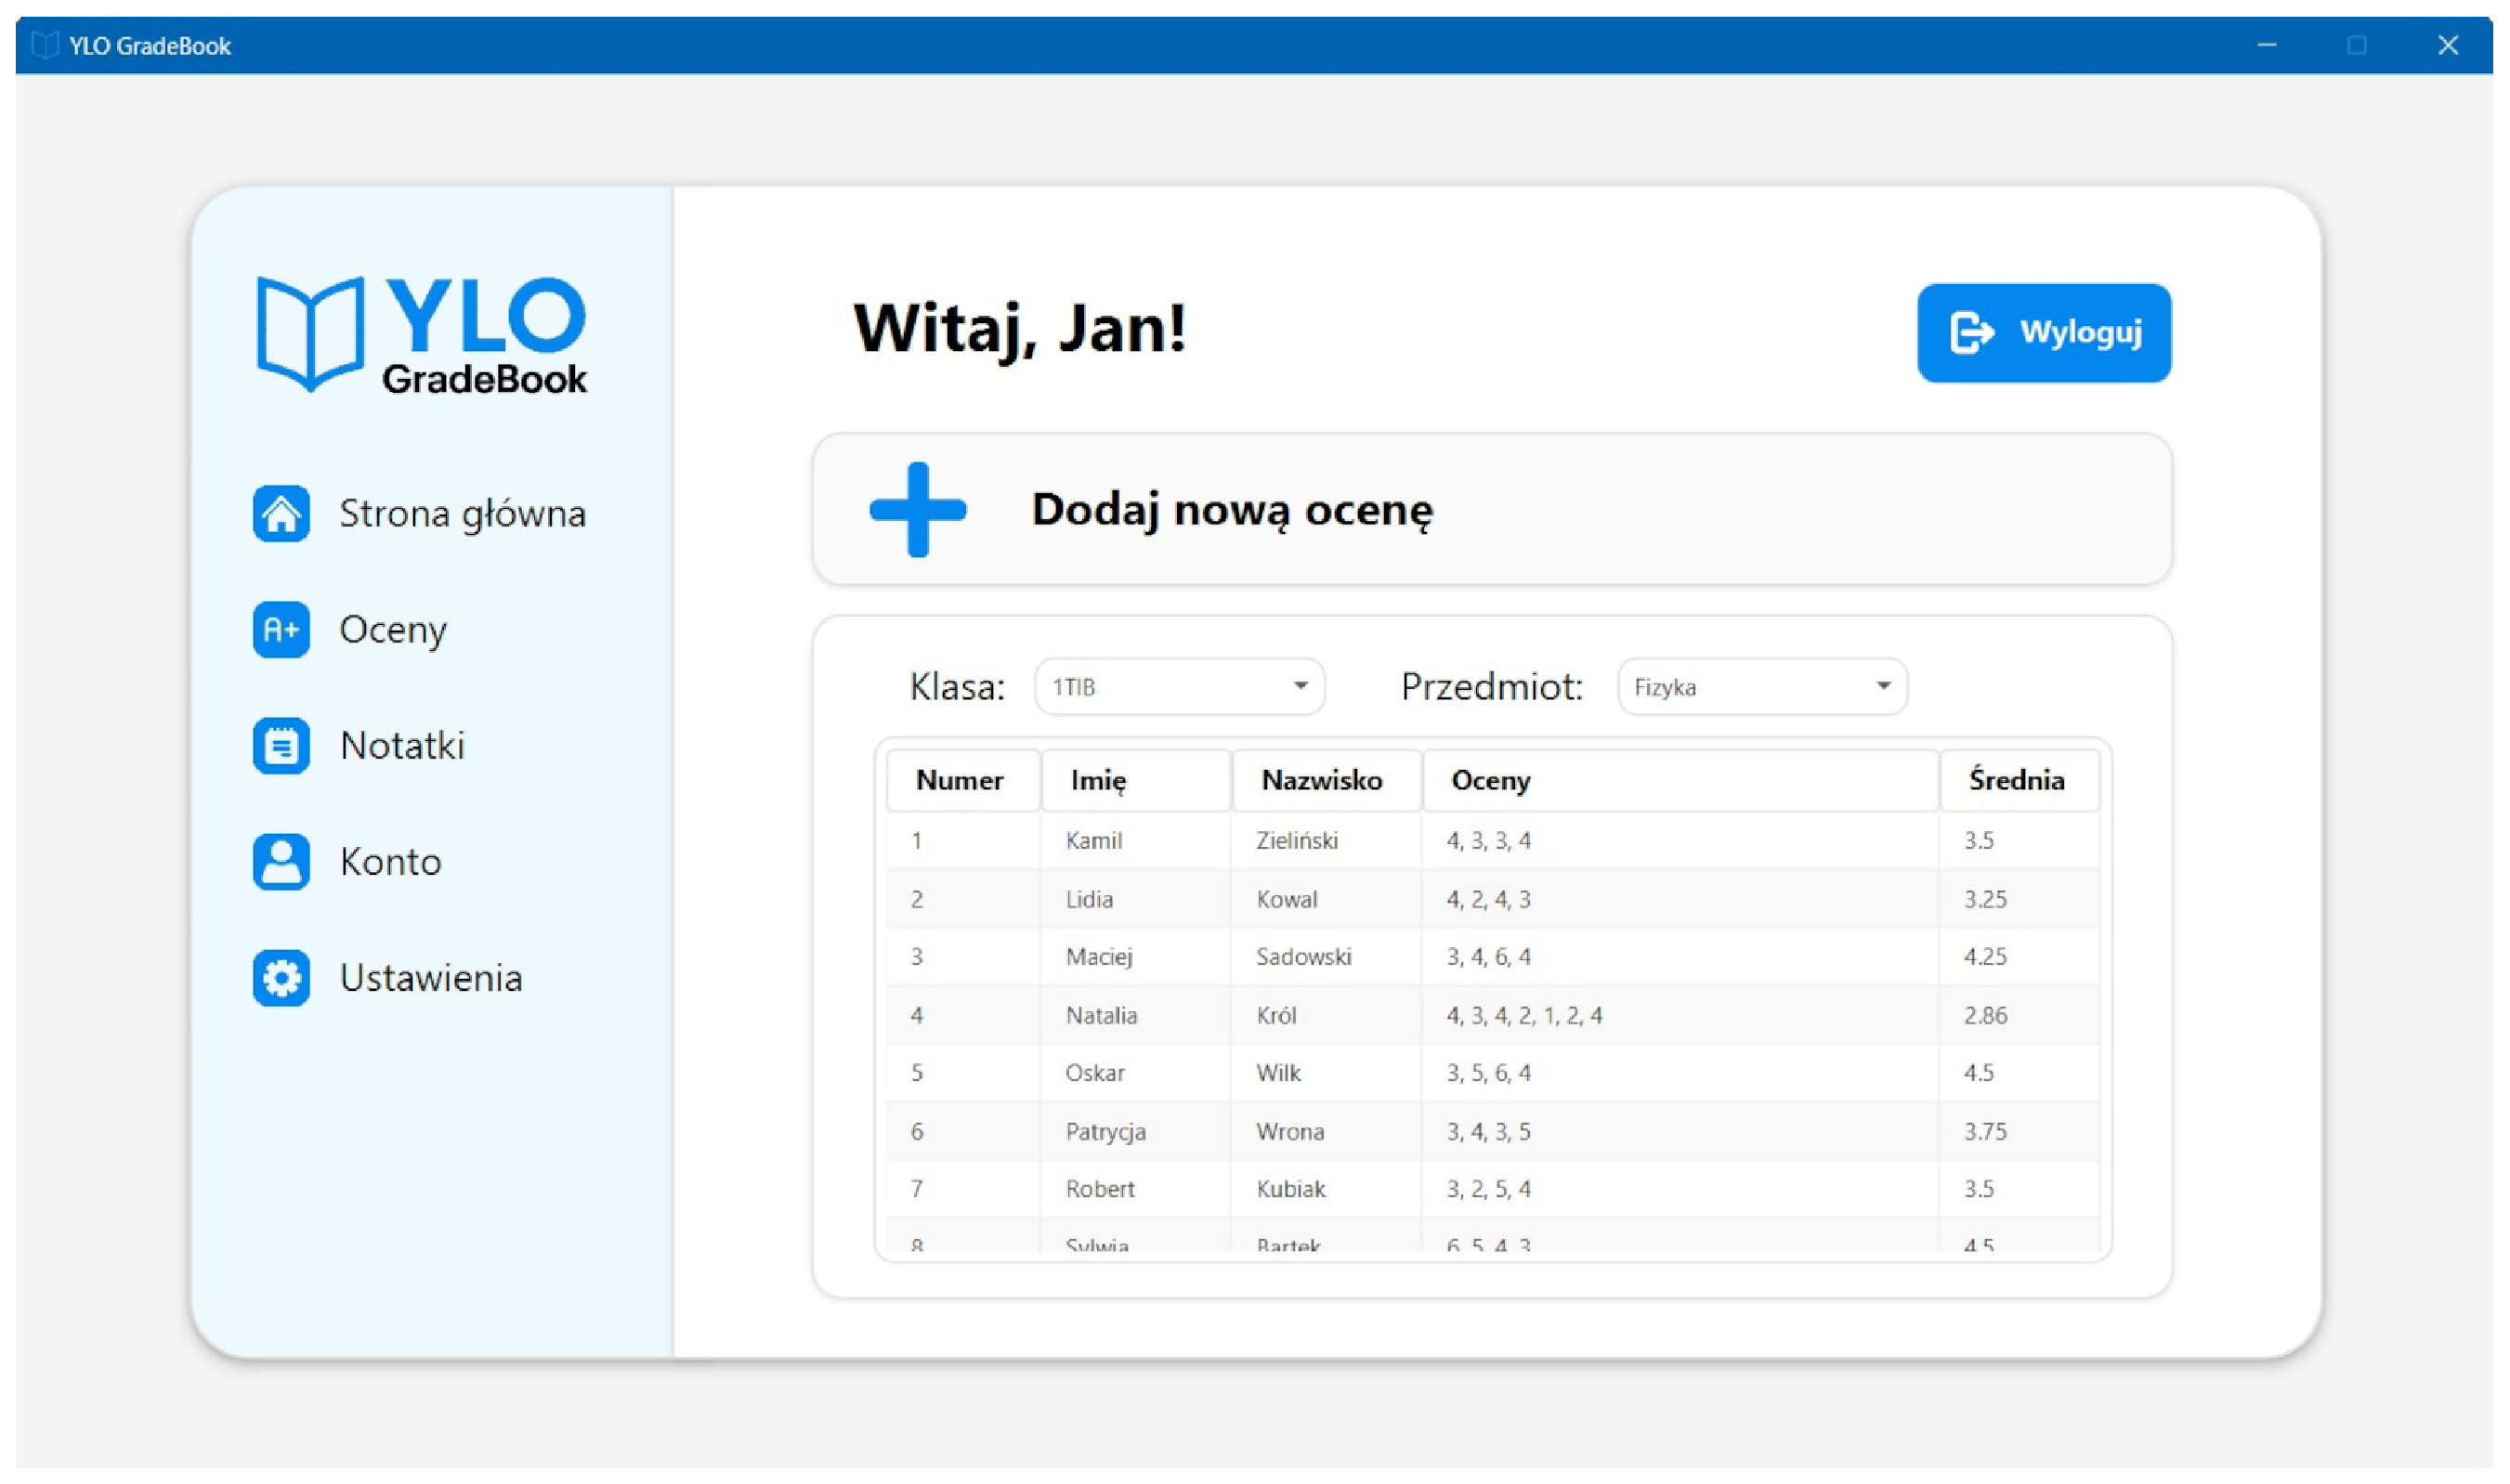
\includegraphics[width=0.9\textwidth]{figures/TeacherWindow/fig_0012.eps}
    \caption{Okno nauczyciela - Zakładka „Oceny”}
    \label{fig:teacherGradePane}
\end{figure}


\newpage
\subsection{Pozostałe zakładki}
Poniżej przedstawiono listę zakładek, które posiadają identyczną budowę, niezależnie od roli zalogowanego użytkownika.

\subsubsection{Zakładka „Notatki”}
Widok zawiera przycisk umożliwiający otwarcie okna typu pop-up, w którym użytkownik może dodać własną notatkę osobistą. Obok znajduje się również przycisk służący do odświeżania tabeli prezentującej wszystkie notatki przypisane do jego konta. Przy każdym rekodzie dodano przycisk textbf{Usuń}, który umożliwia usunięcie notatki z tabeli oraz z bazy danych.
\begin{figure}[H]
    \centering
    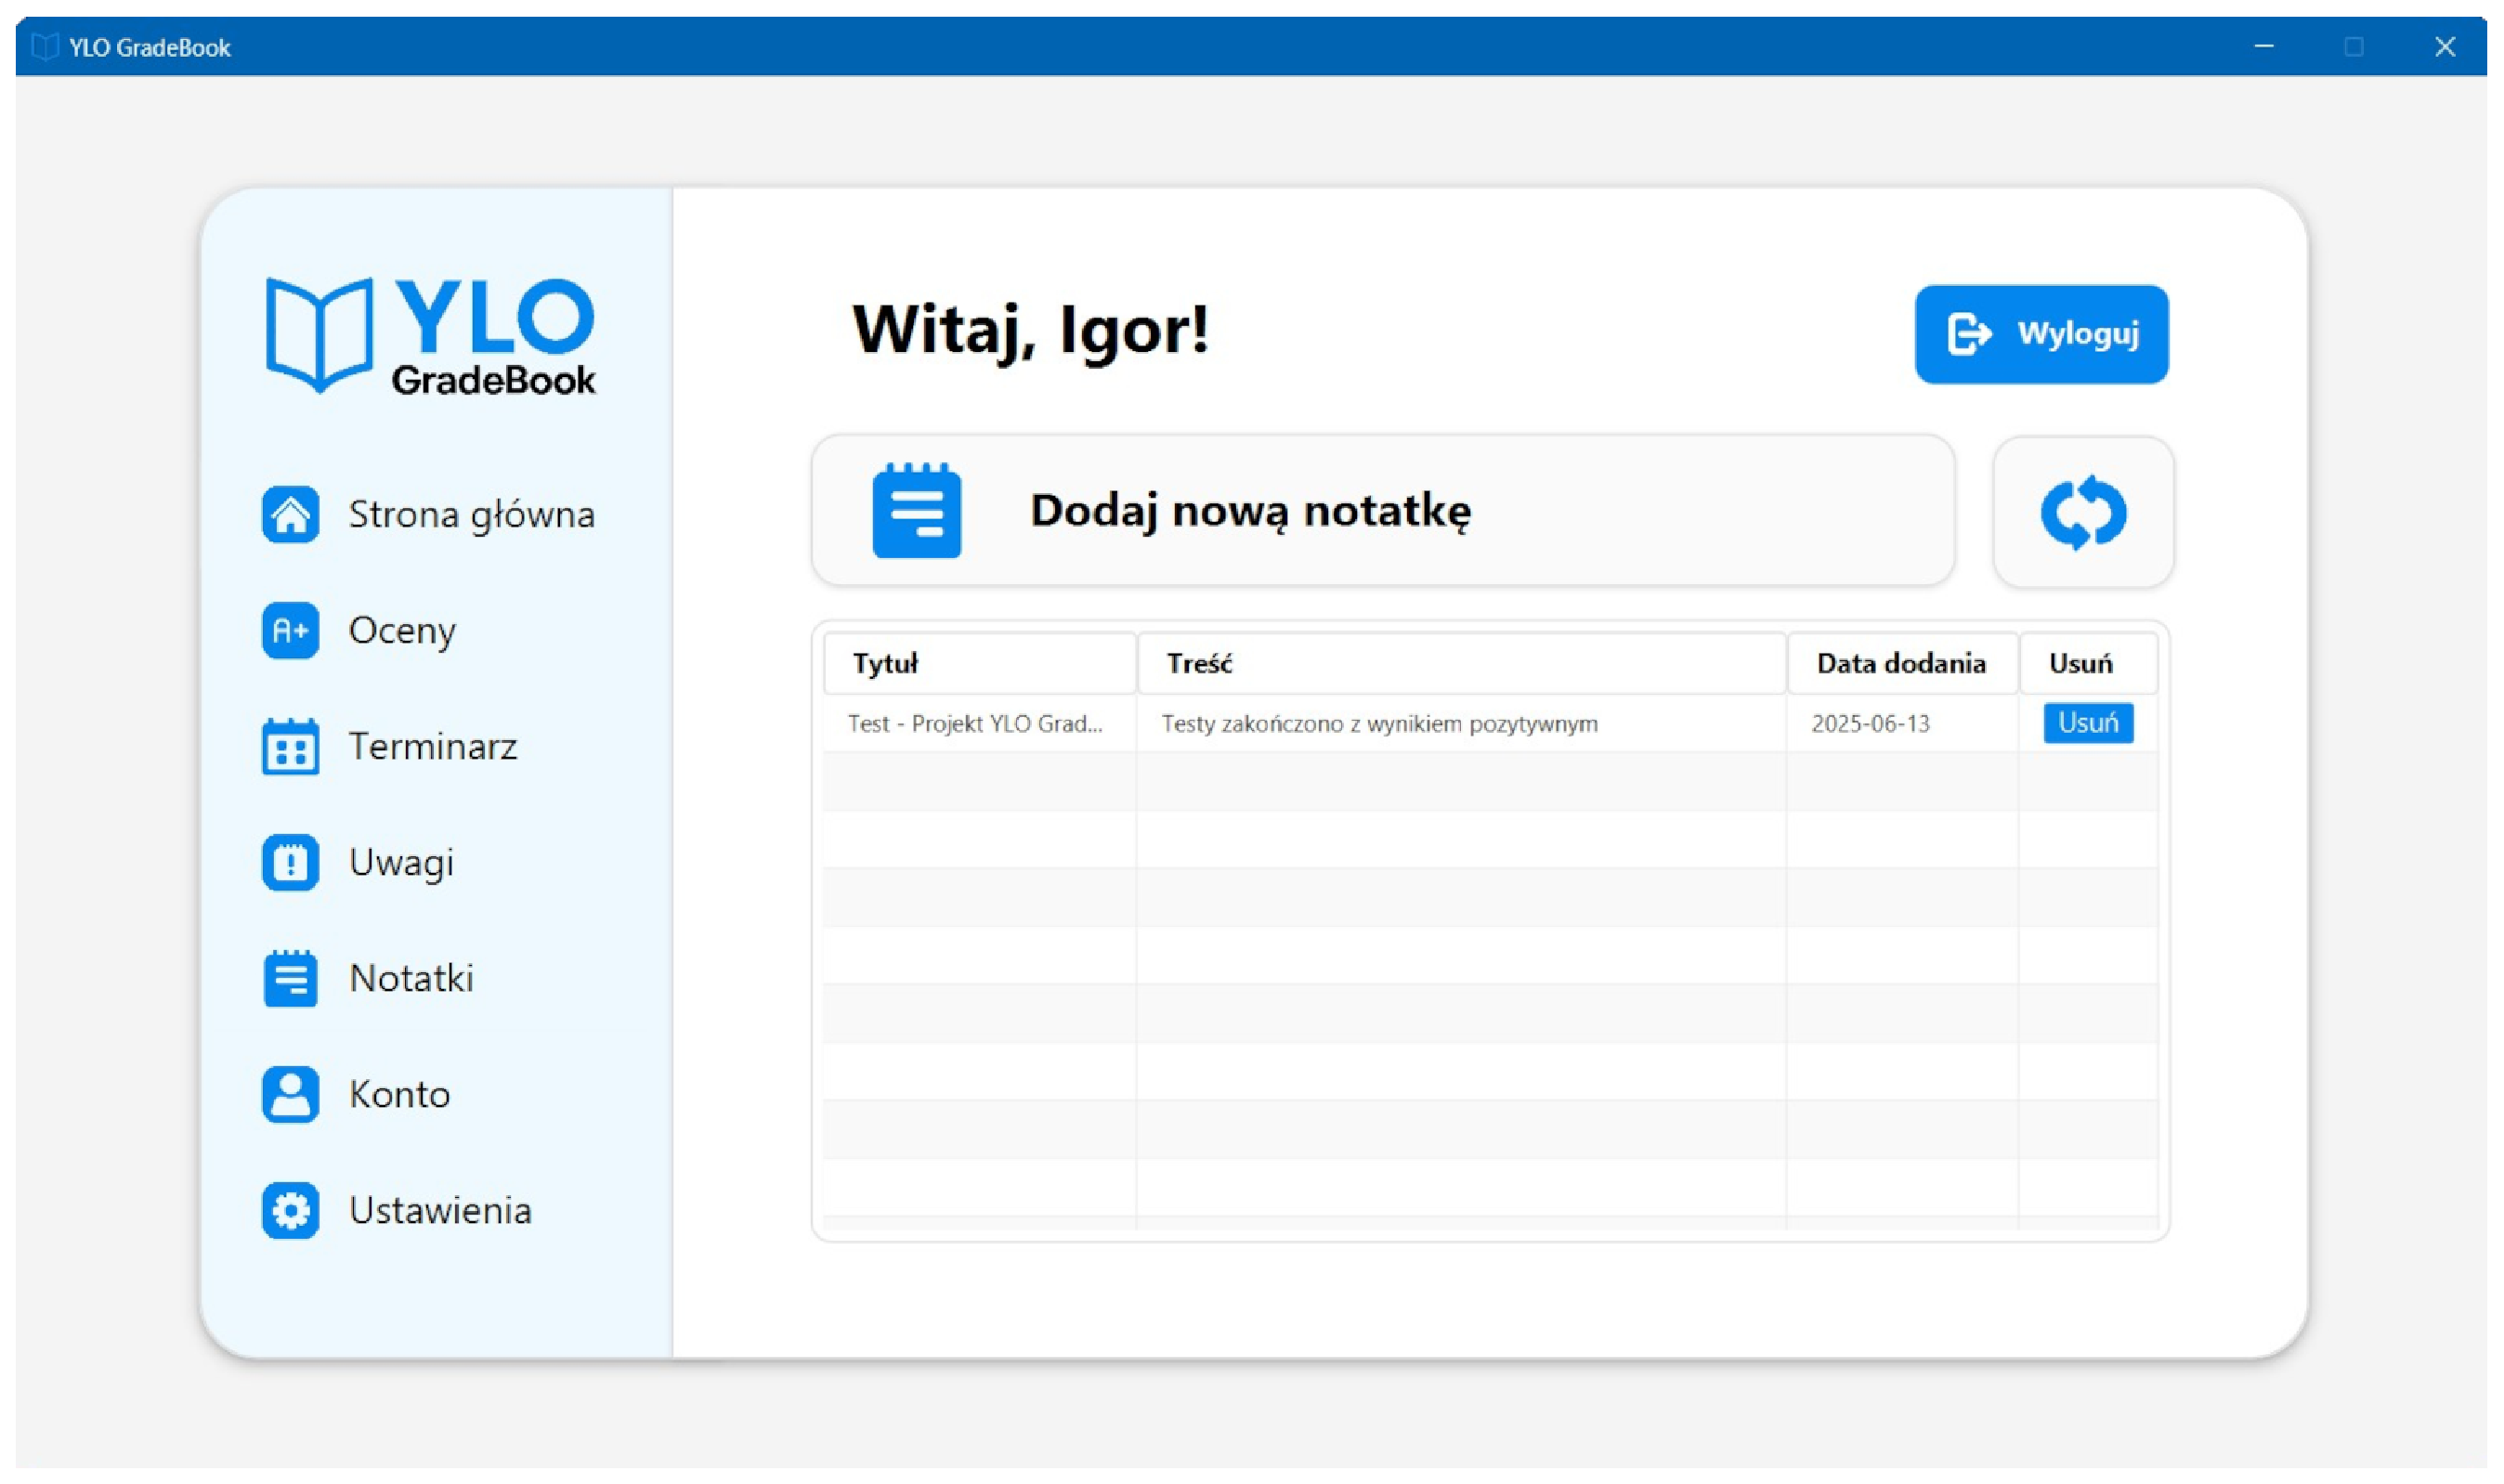
\includegraphics[width=0.9\textwidth]{figures/StudentWindow/fig_0013.eps}
    \caption{Okno ucznia - Zakładka „Notatki”}
    \label{fig:studentNotesPane}
\end{figure}
\newpage
\subsubsection{Zakładka „Konto”}
Widok pozwala na wyświetlenie danych użytkownika aktualnie zalogowanego do systemu.
\begin{figure}[H]
    \centering
    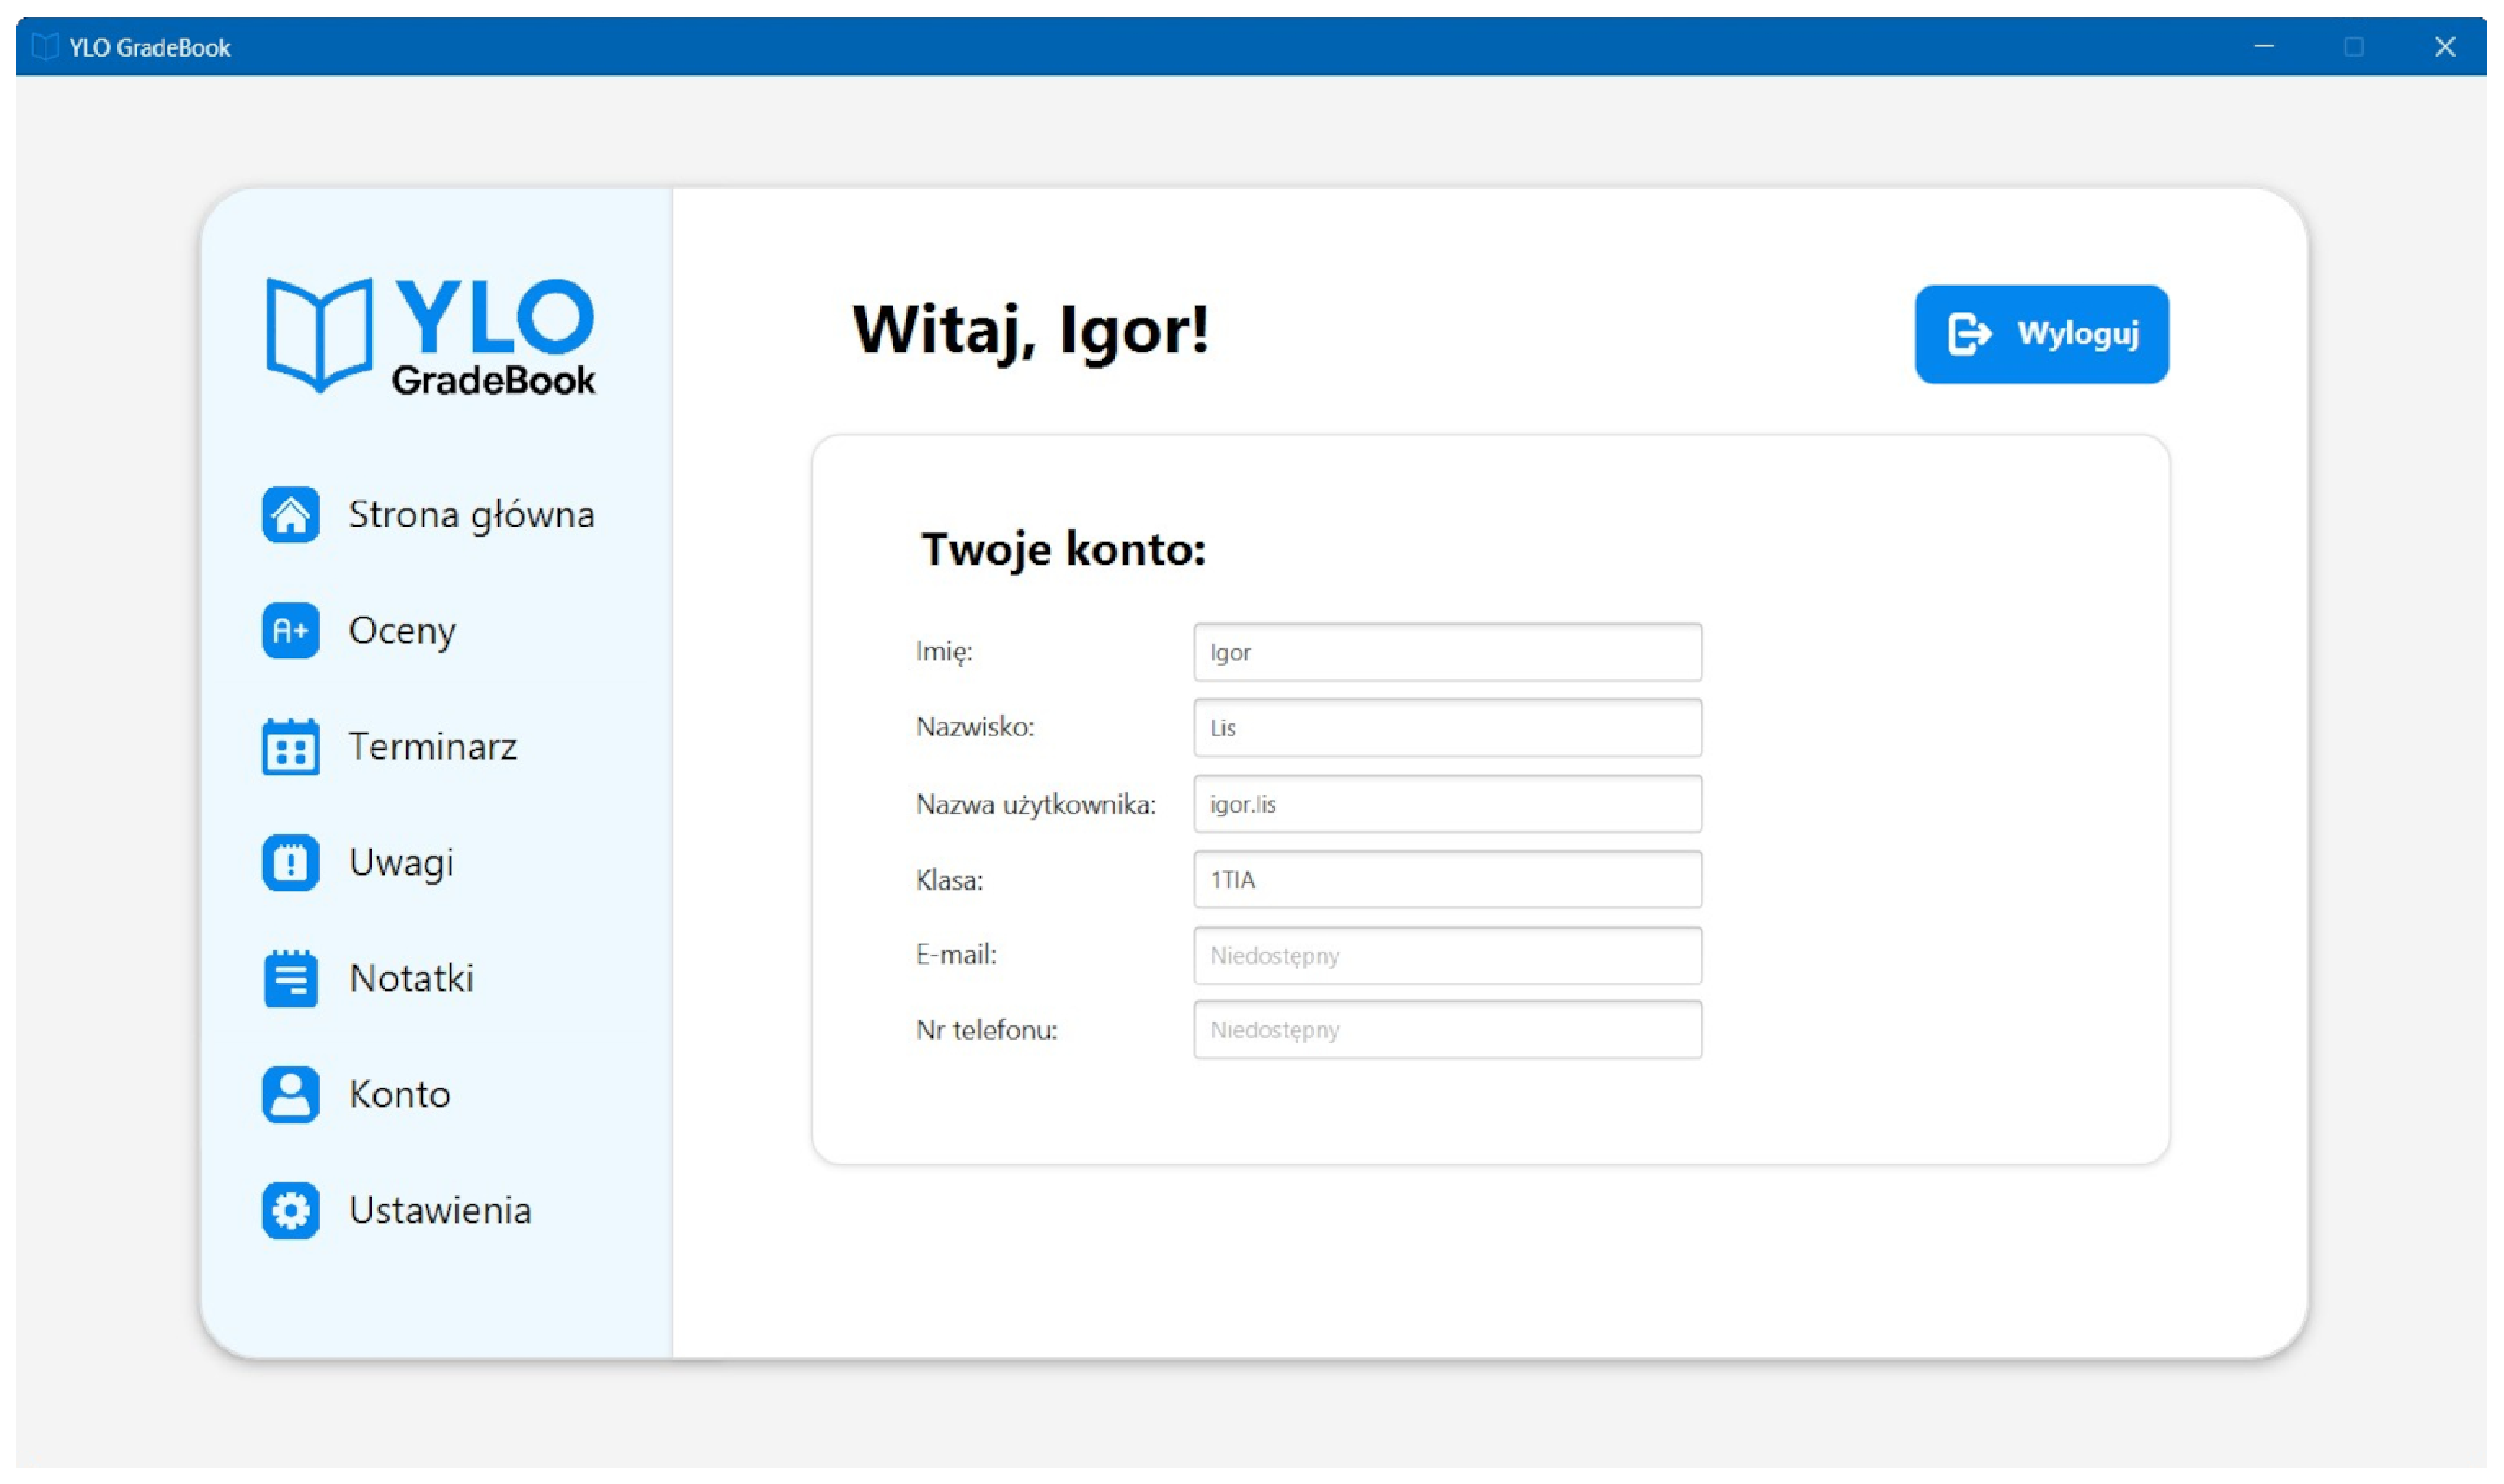
\includegraphics[width=0.9\textwidth]{figures/StudentWindow/fig_0014.eps}
    \caption{Zakładka „Konto”}
    \label{fig:accountPane}
\end{figure}

\subsubsection{Zakładka „Ustawienia”}
Ostatnia zakładka umożliwia użytkownikowi zarządzanie jego danymi konta. Zawiera przycisk uruchamiający okno resetowania hasła oraz przycisk przygotowany pod planowaną funkcję zmiany adresu e-mail przypisanego do profilu użytkownika.
\begin{figure}[H]
    \centering
    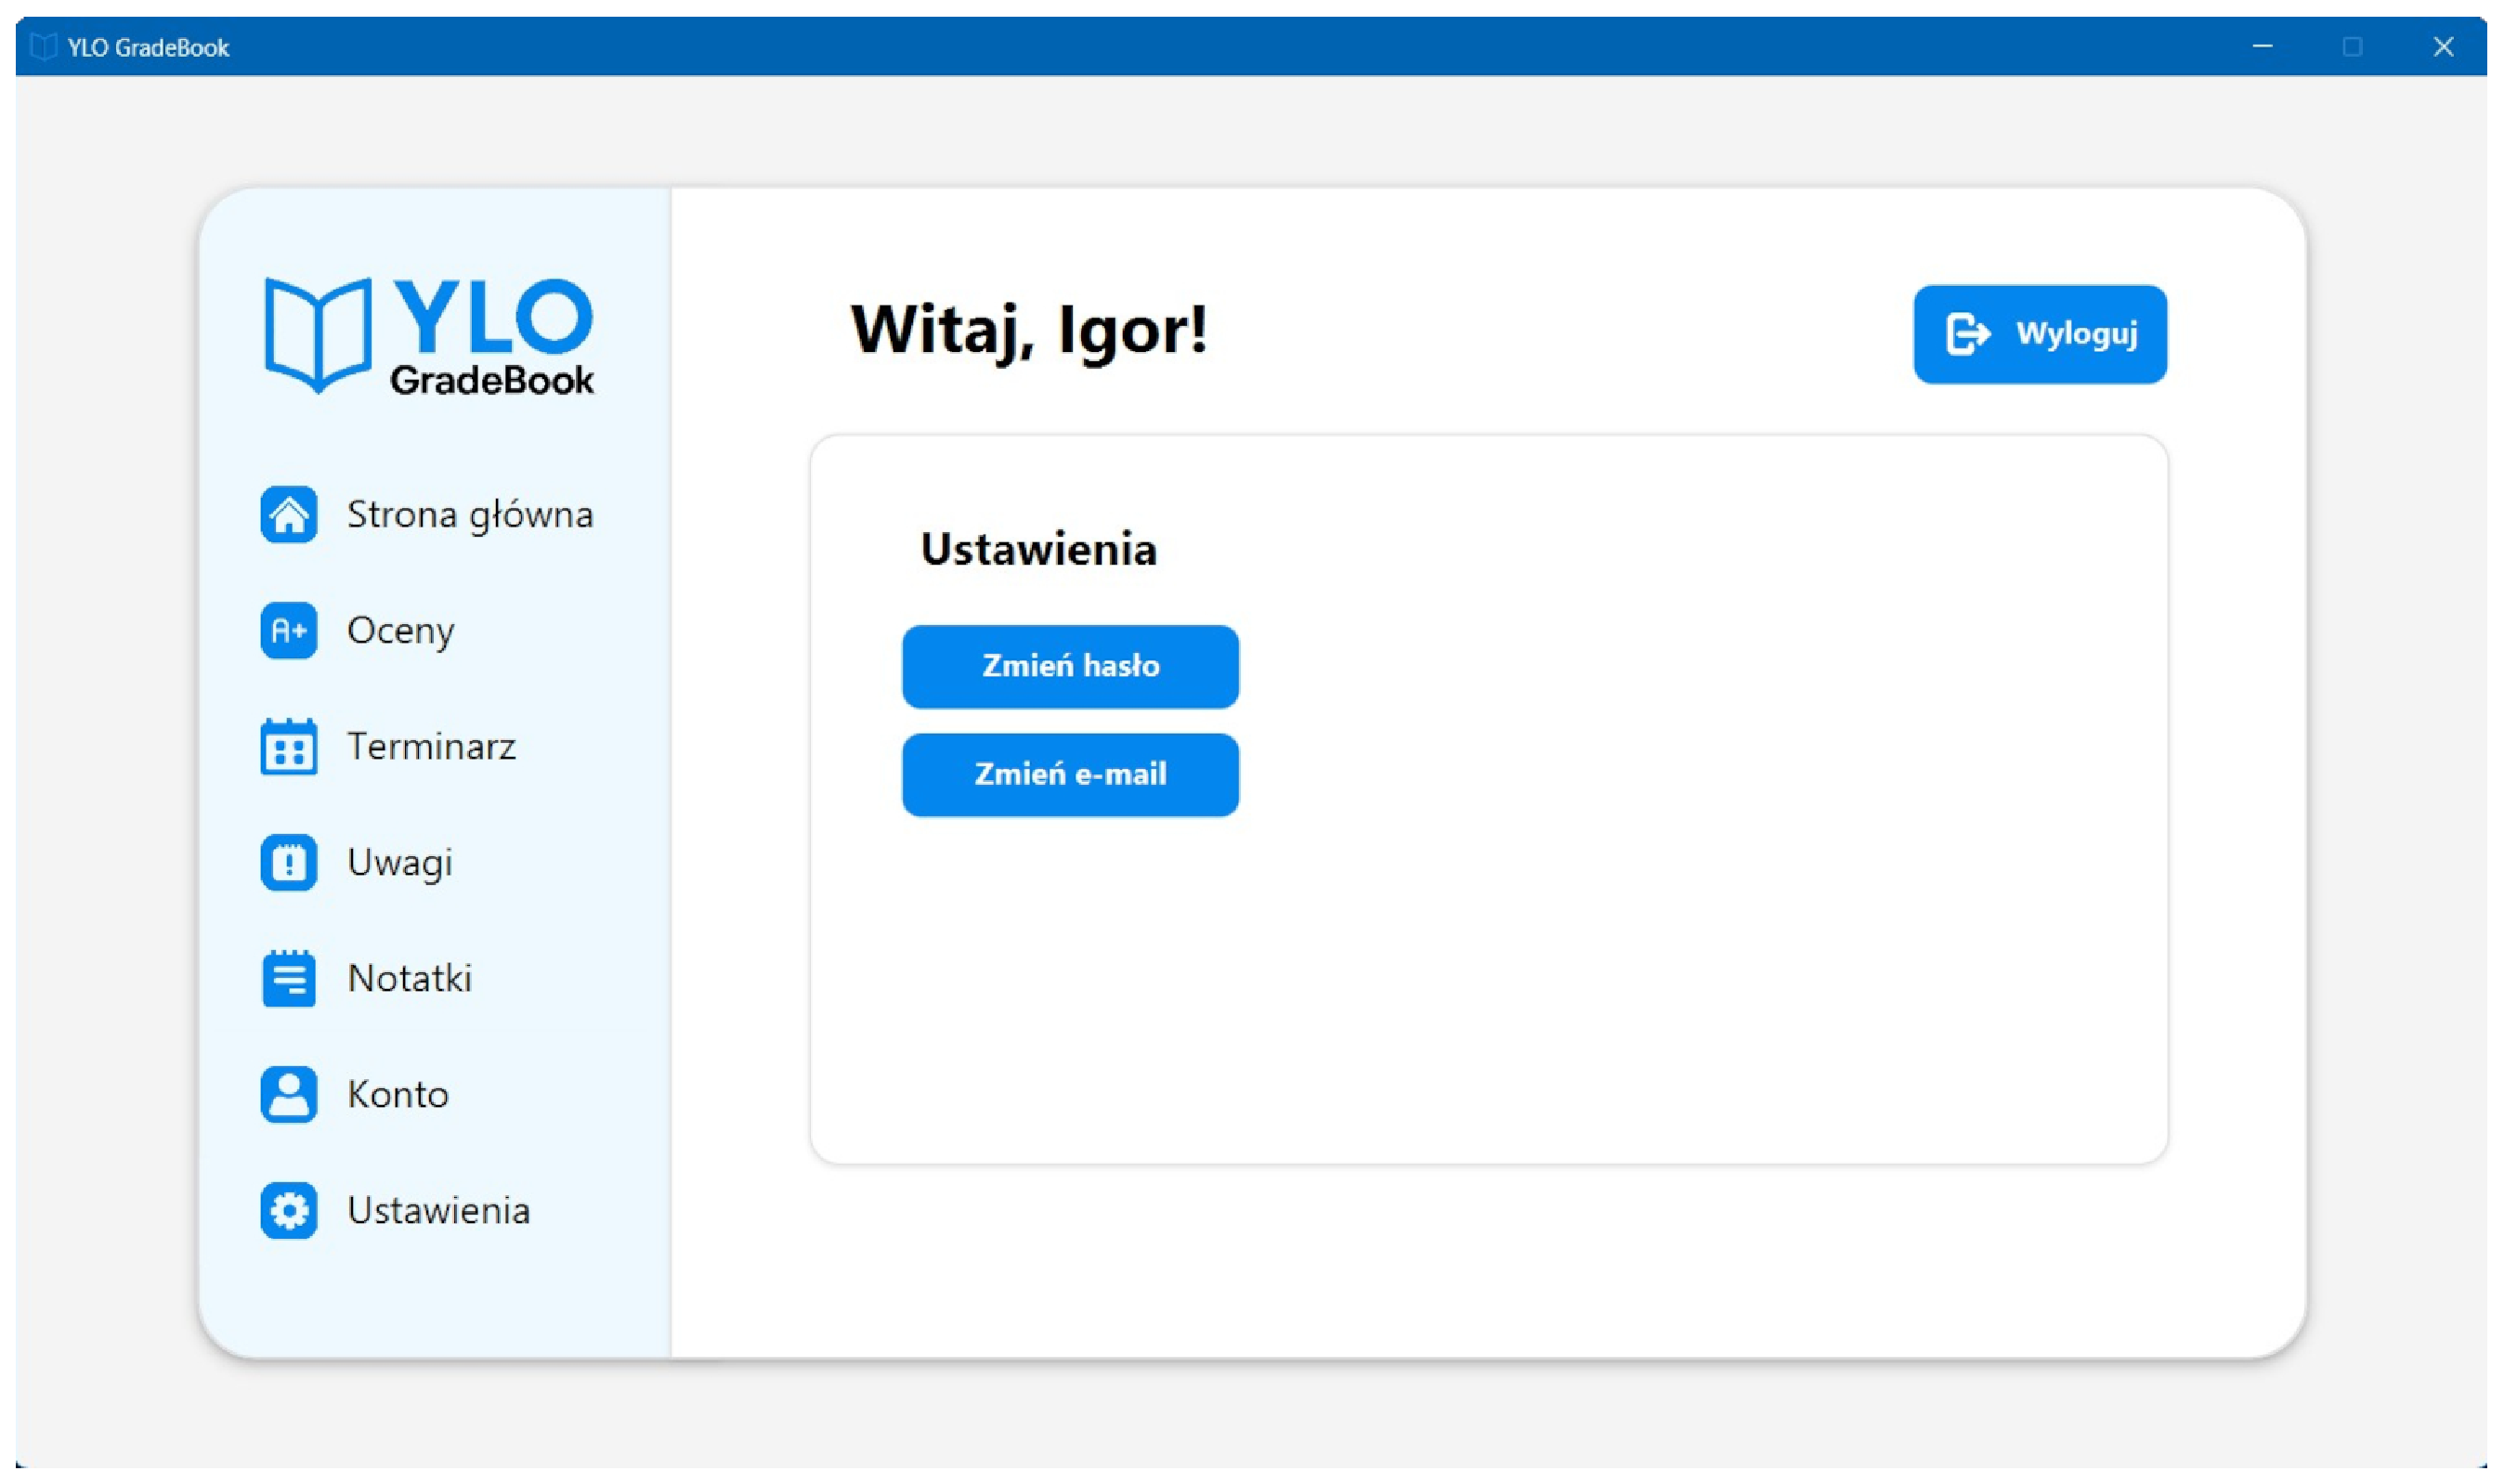
\includegraphics[width=0.9\textwidth]{figures/StudentWindow/fig_0015.eps}
    \caption{Zakładka „Ustawienia”}
    \label{fig:settingsPane}
\end{figure}

\subsection{Widok okna PopUp}
Widok ten służy do wyświetlenia formularza umożliwiającego dodanie nowych danych do systemu.
W zależności od kontekstu, posiada cztery różne wersje, z których każda odpowiada innej funkcji (np. dodawanie ocen, uwagi, terminu lub notatki).
\begin{itemize}
    \item Każda wersja zawiera pola do wprowadzania odpowiednich danych oraz przycisk umożliwiający dodanie ich do bazy danych.
    \item W przypadku błędnego wypełnienia formularza, system wyświetla odpowiedni komunikat walidacyjny.
    \item Po zatwierdzeniu formularza pojawia się komunikat informujący o rezultacie operacji — czy została wykonana pomyślnie, czy wystąpił błąd.
\end{itemize}
\clearpage

\subsubsection{Okno PopUp – Dodawanie oceny}

Formularz umożliwia nauczycielowi przypisanie nowej oceny wybranemu uczniowi. Widok zawiera listy rozwijane do wyboru klasy, ucznia, przedmiotu i typu oceny, a także pole do wpisania wartości punktowej.

\begin{figure}[H]
    \centering
    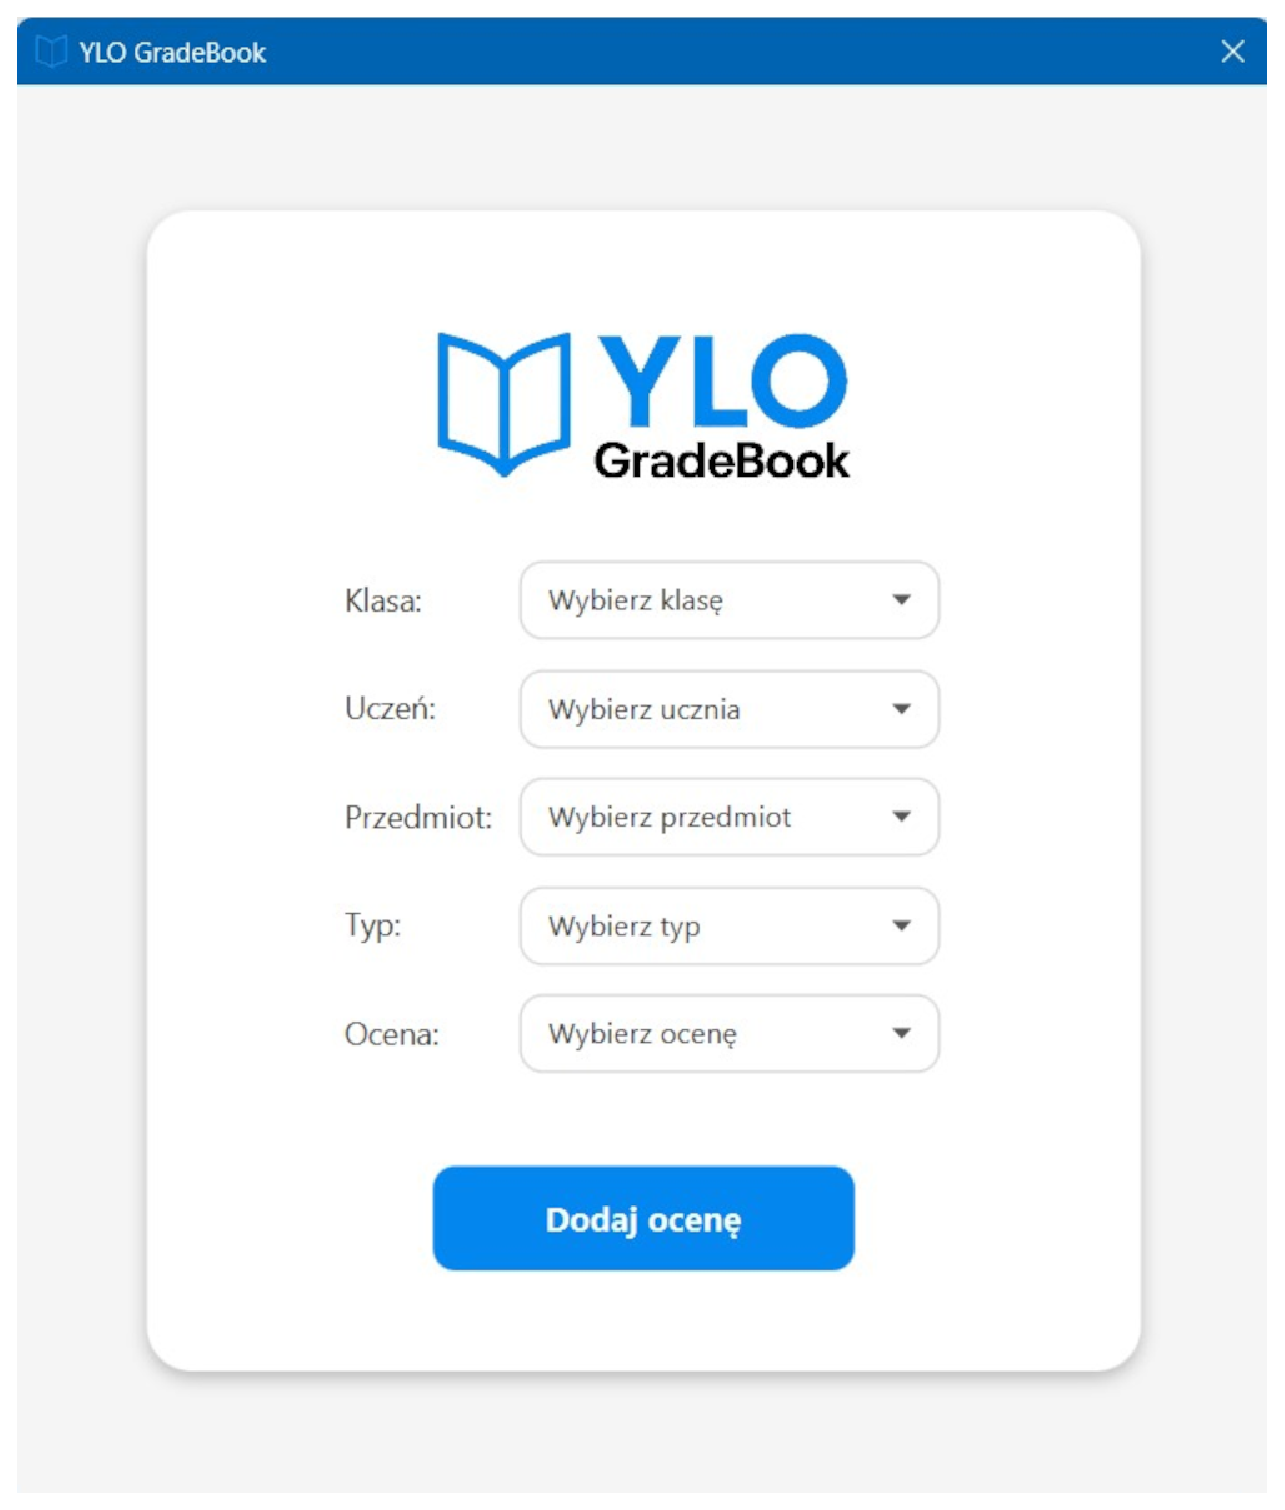
\includegraphics[width=0.9\textwidth]{figures/fig_0016.eps}
    \caption{PopUp — dodawanie nowej oceny}
    \label{fig:popUpGrade}
\end{figure}
\newpage
\subsubsection{Okno PopUp – Dodawanie terminów}

Okno to pozwala nauczycielowi na dodanie nowego wydarzenia (np. sprawdzianu, zadania) przypisanego do konkretnej klasy i przedmiotu. Użytkownik wybiera datę oraz podaje krótki opis.

\begin{figure}[H]
    \centering
    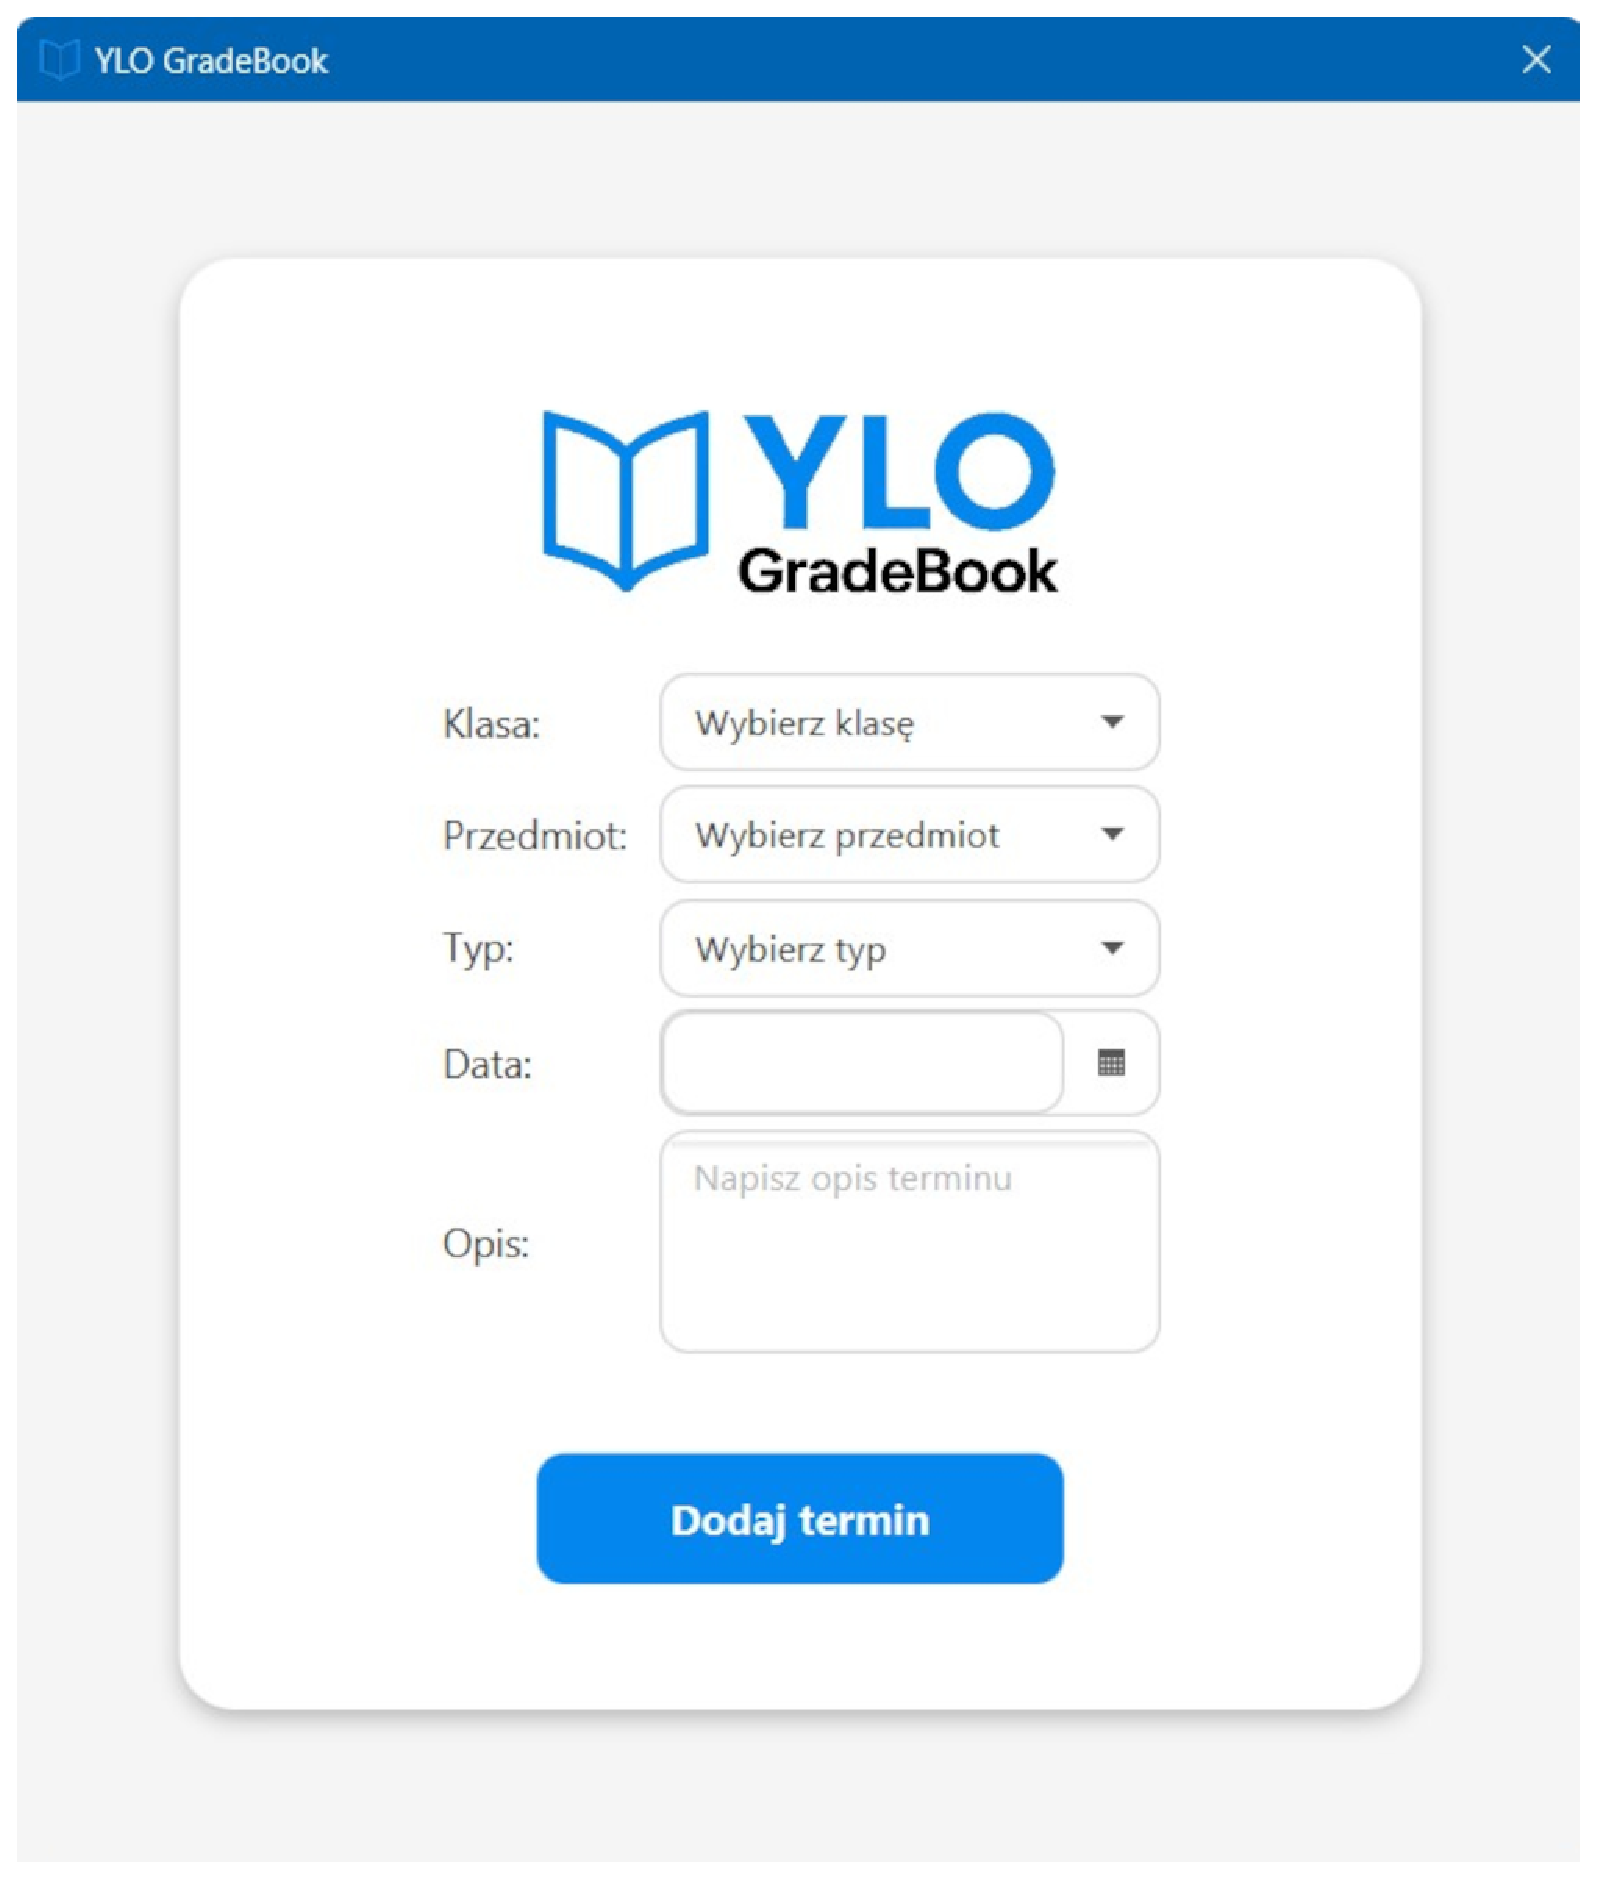
\includegraphics[width=0.9\textwidth]{figures/fig_0017.eps}
    \caption{PopUp — dodawanie nowego terminu}
    \label{fig:popUpDeadLine}
\end{figure}
\newpage
\subsubsection{Okno PopUp – Dodawanie uwag}

Formularz służy do wystawiania uwag punktowych uczniom. Nauczyciel wybiera ucznia, wprowadza liczbę punktów oraz wpisuje treść ograniczoną do 60 znaków.

\begin{figure}[H]
    \centering
    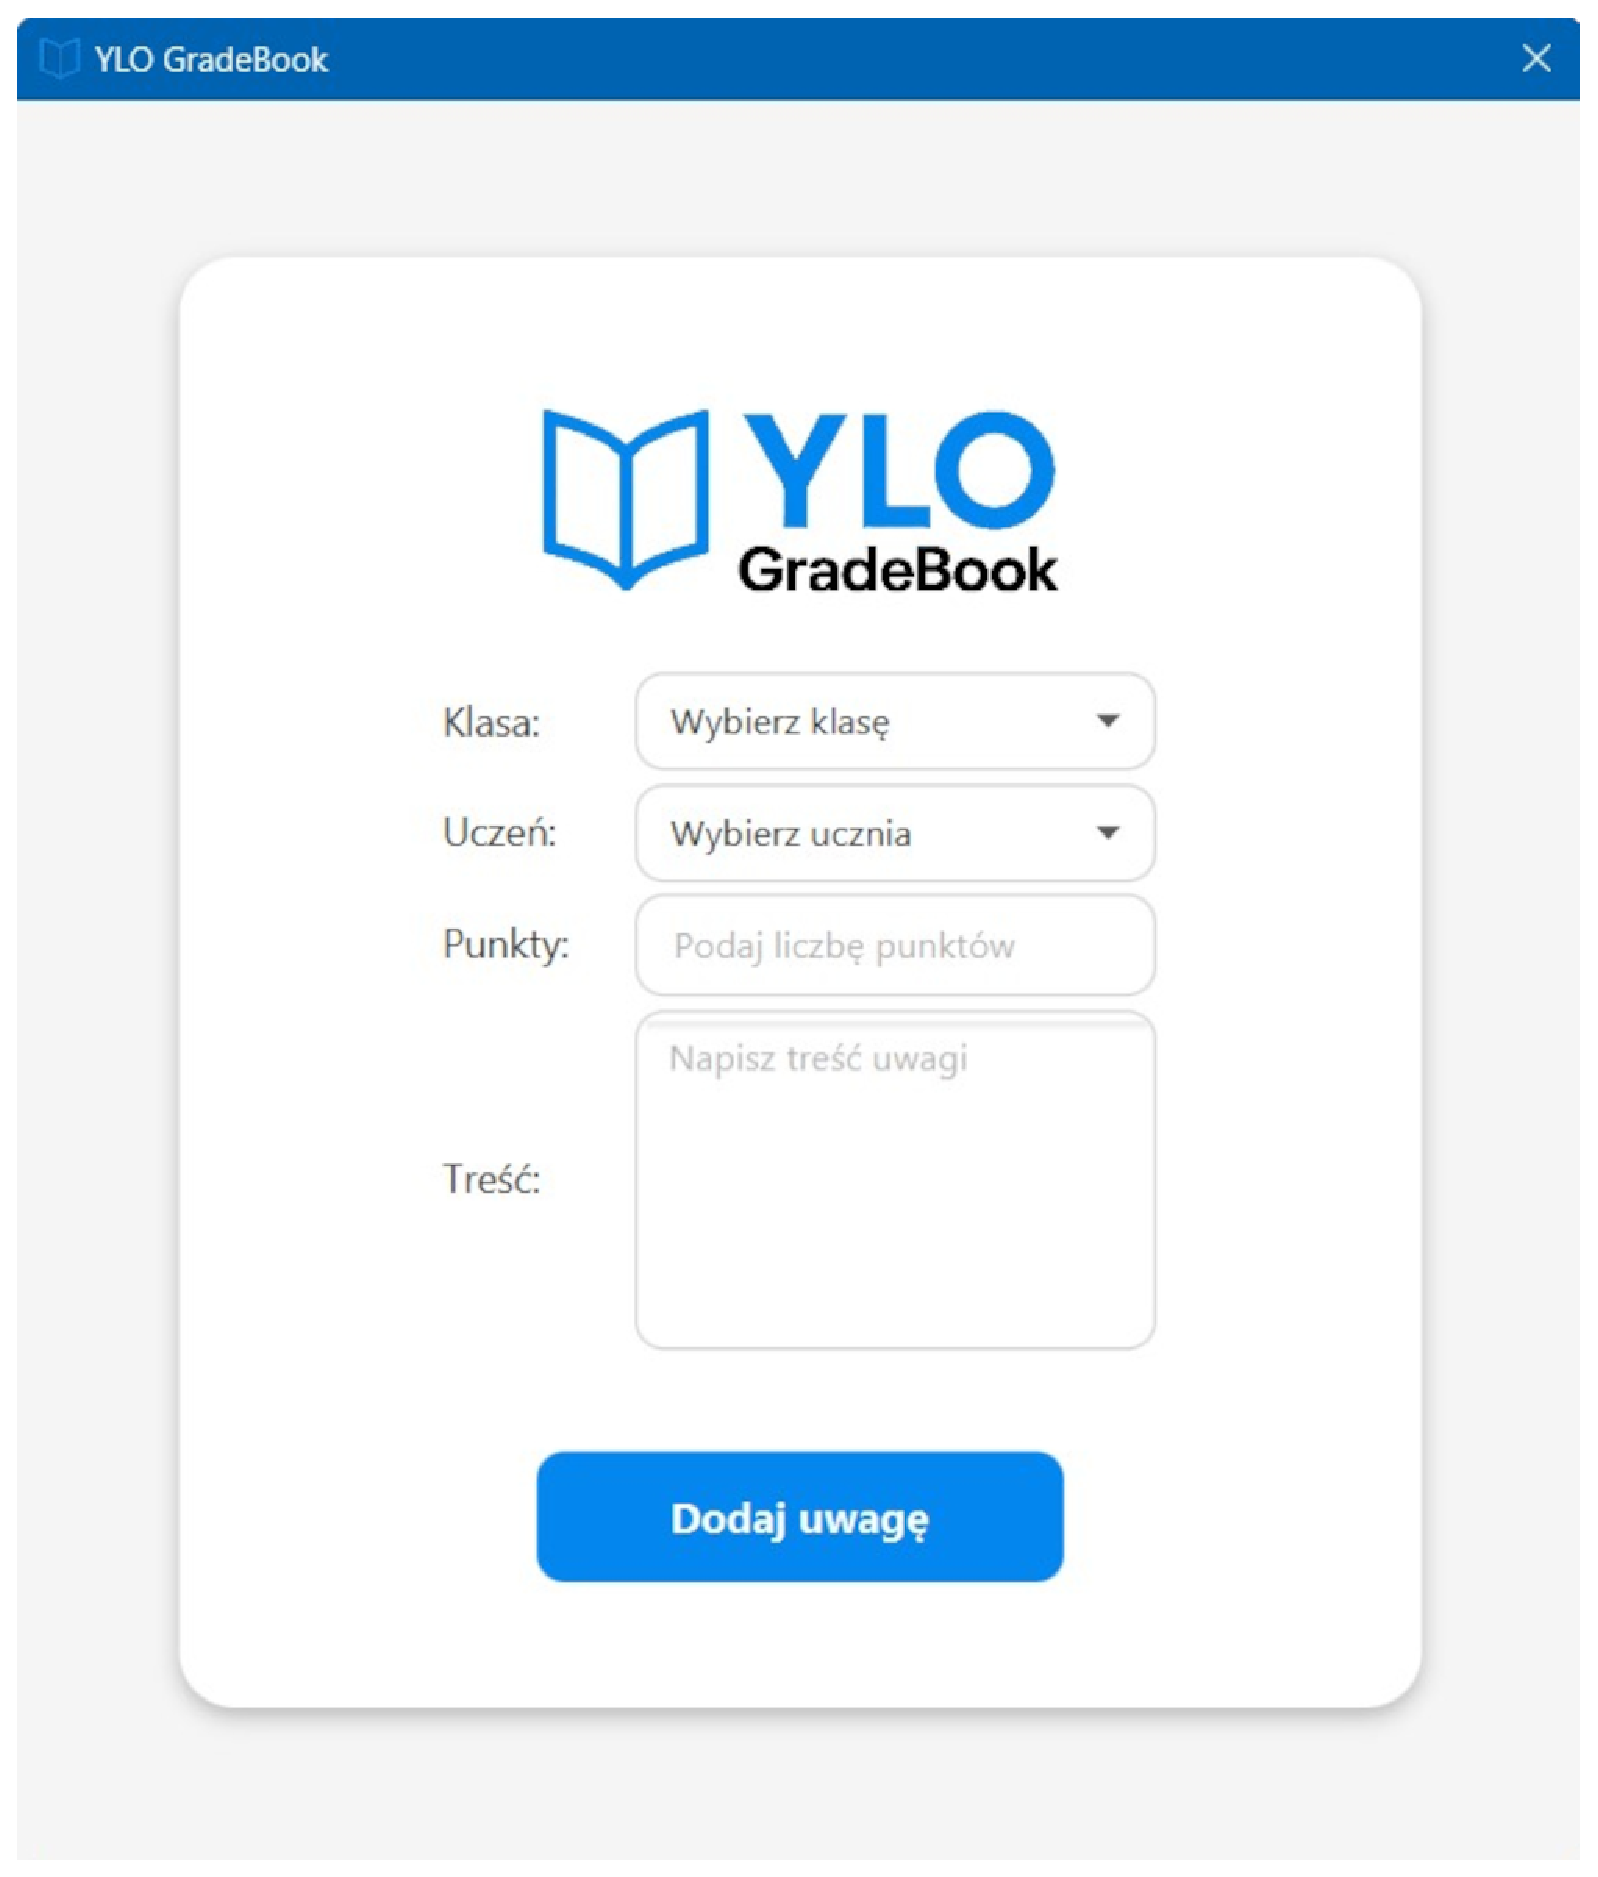
\includegraphics[width=0.9\textwidth]{figures/fig_0018.eps}
    \caption{PopUp — dodawanie uwagi uczniowi}
    \label{fig:popUpNN}
\end{figure}
\newpage
\subsubsection{Okno PopUp – Dodawanie notatek}
Widok umożliwia dodanie osobistej notatki. Użytkownik podaje tytuł oraz treść, a następnie zapisuje ją w systemie — notatka przypisywana jest automatycznie do jego konta.

\begin{figure}[H]
    \centering
    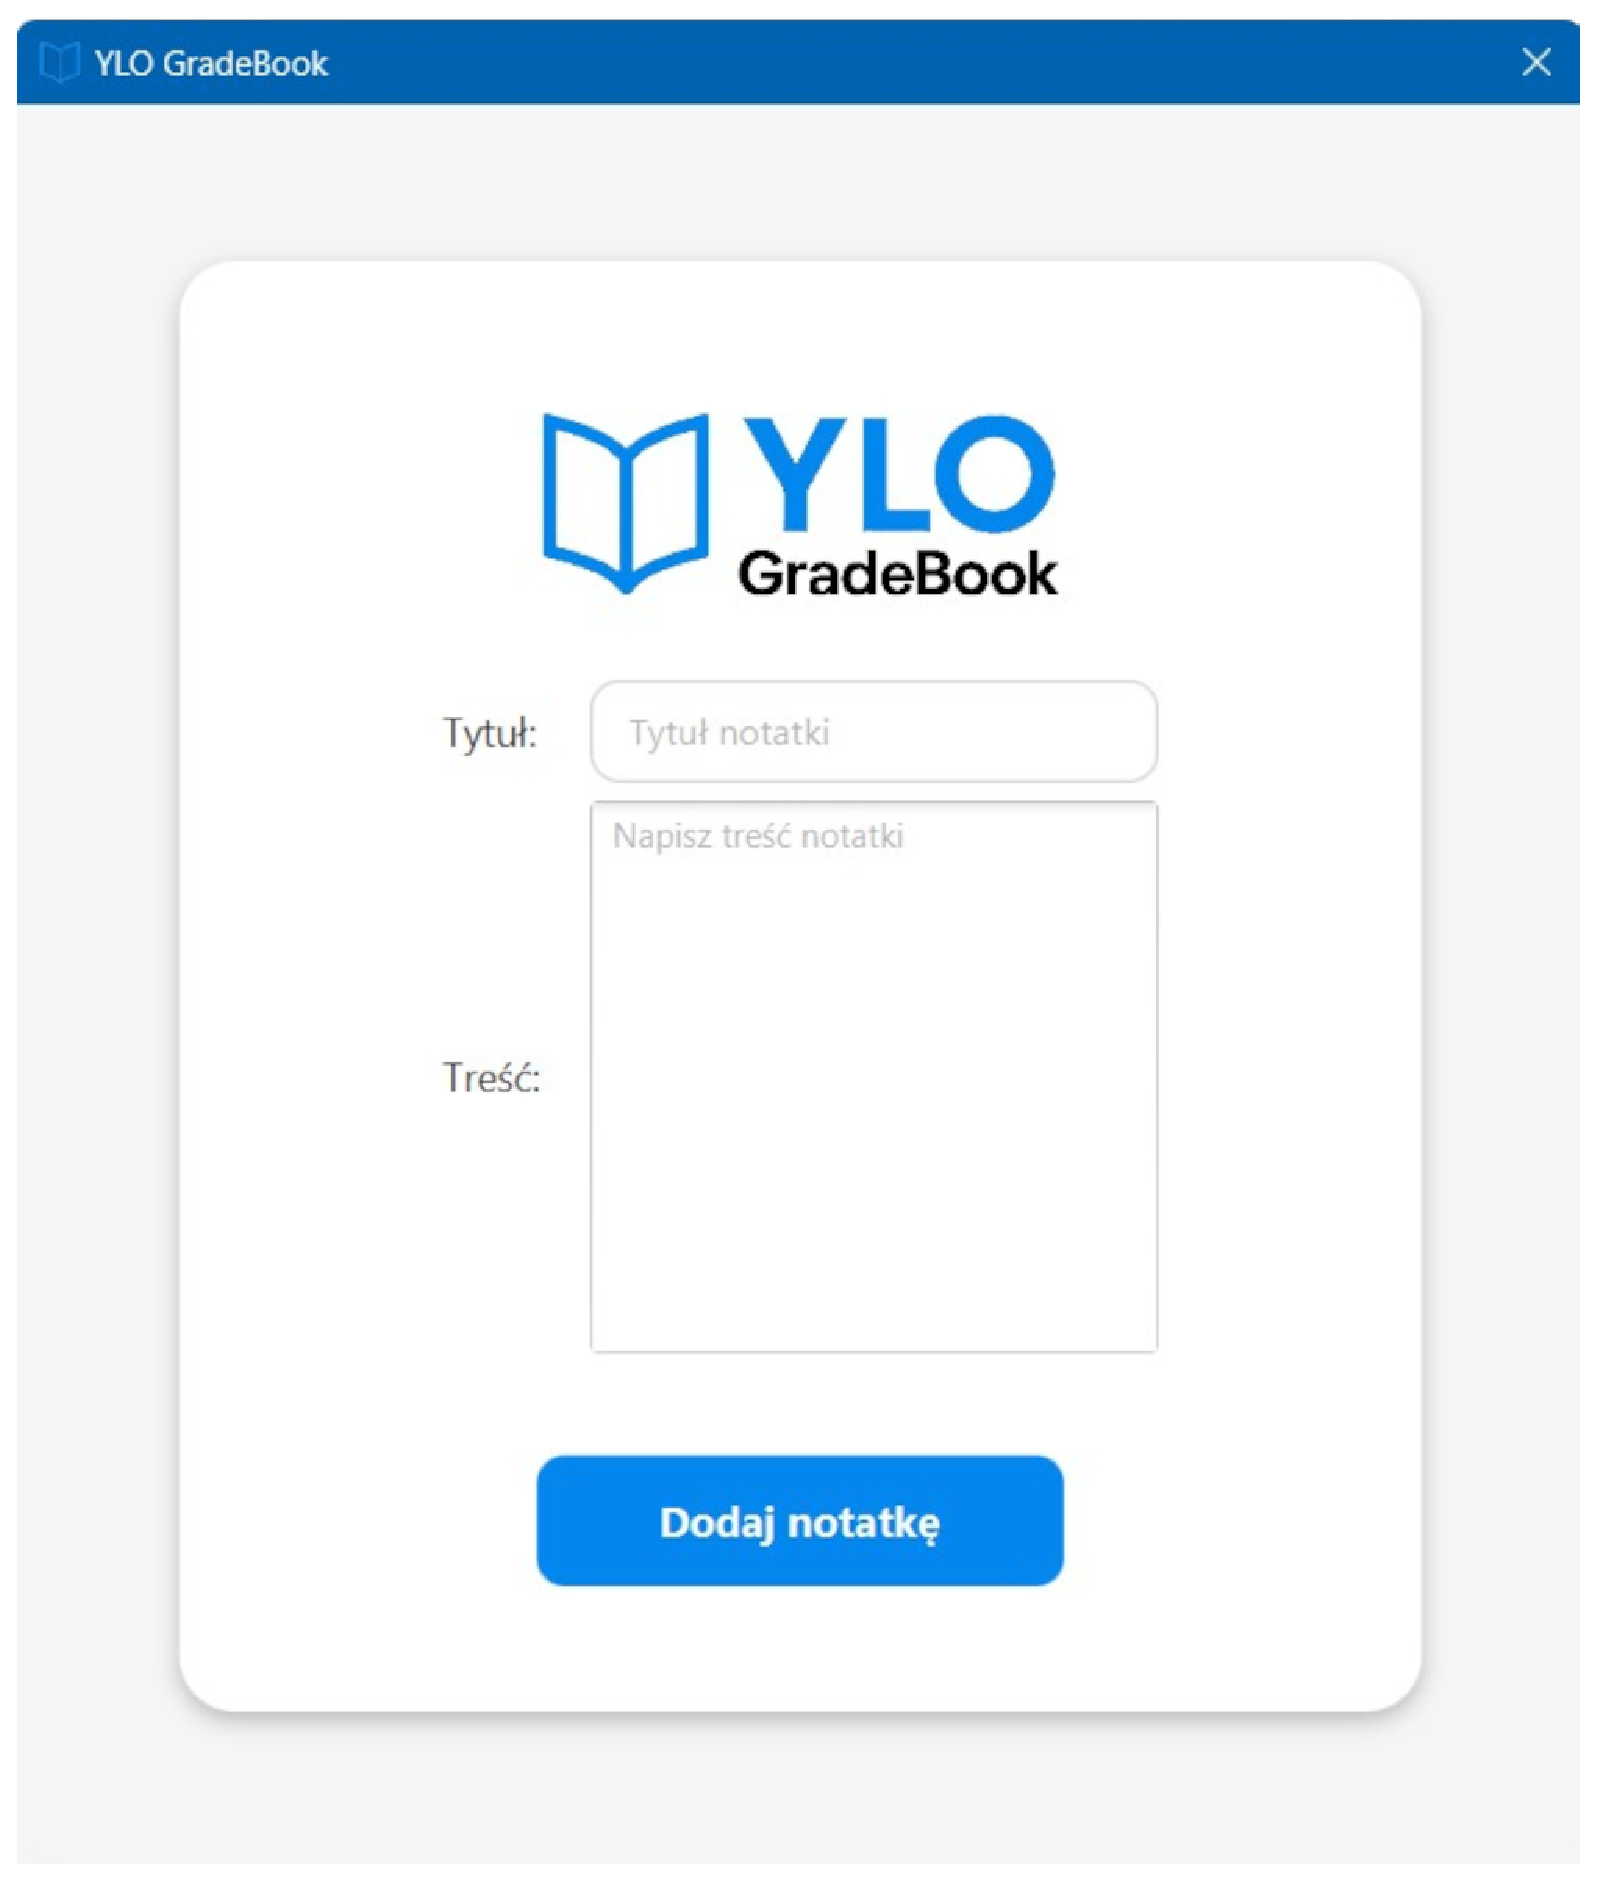
\includegraphics[width=0.9\textwidth]{figures/fig_0019.eps}
    \caption{PopUp — dodawanie notatki}
    \label{fig:popUpNote}
\end{figure}
\newpage
\section{Mechanizm alertów systemowych}

Aplikacja \texttt{YLO GradeBook} została wyposażona w system alertów, który informuje użytkownika o rezultacie wykonywanej operacji. Komunikaty pojawiają się m.in. przy:

\begin{itemize}
    \item nieprawidłowym logowaniu,
    \item błędnym wypełnieniu formularzy,
    \item anulowaniu operacji,
    \item wylogowaniu z sytemu,
\end{itemize}

Funkcjonalność ta została zrealizowana w klasie bazowej \texttt{SessionController}, która udostępnia wspólne metody. Dzięki ich zastosowaniu interfejs użytkownika informuje o przebiegu operacji w sposób przejrzysty, spójny i natychmiastowy.

Rozwiązanie to znacząco podnosi komfort i poczucie bezpieczeństwa przy wprowadzaniu danych do systemu.

Poniżej przedstawiono jeden z alertów pojawiających się podczas próby logowania.
\begin{figure}[H]
    \centering
    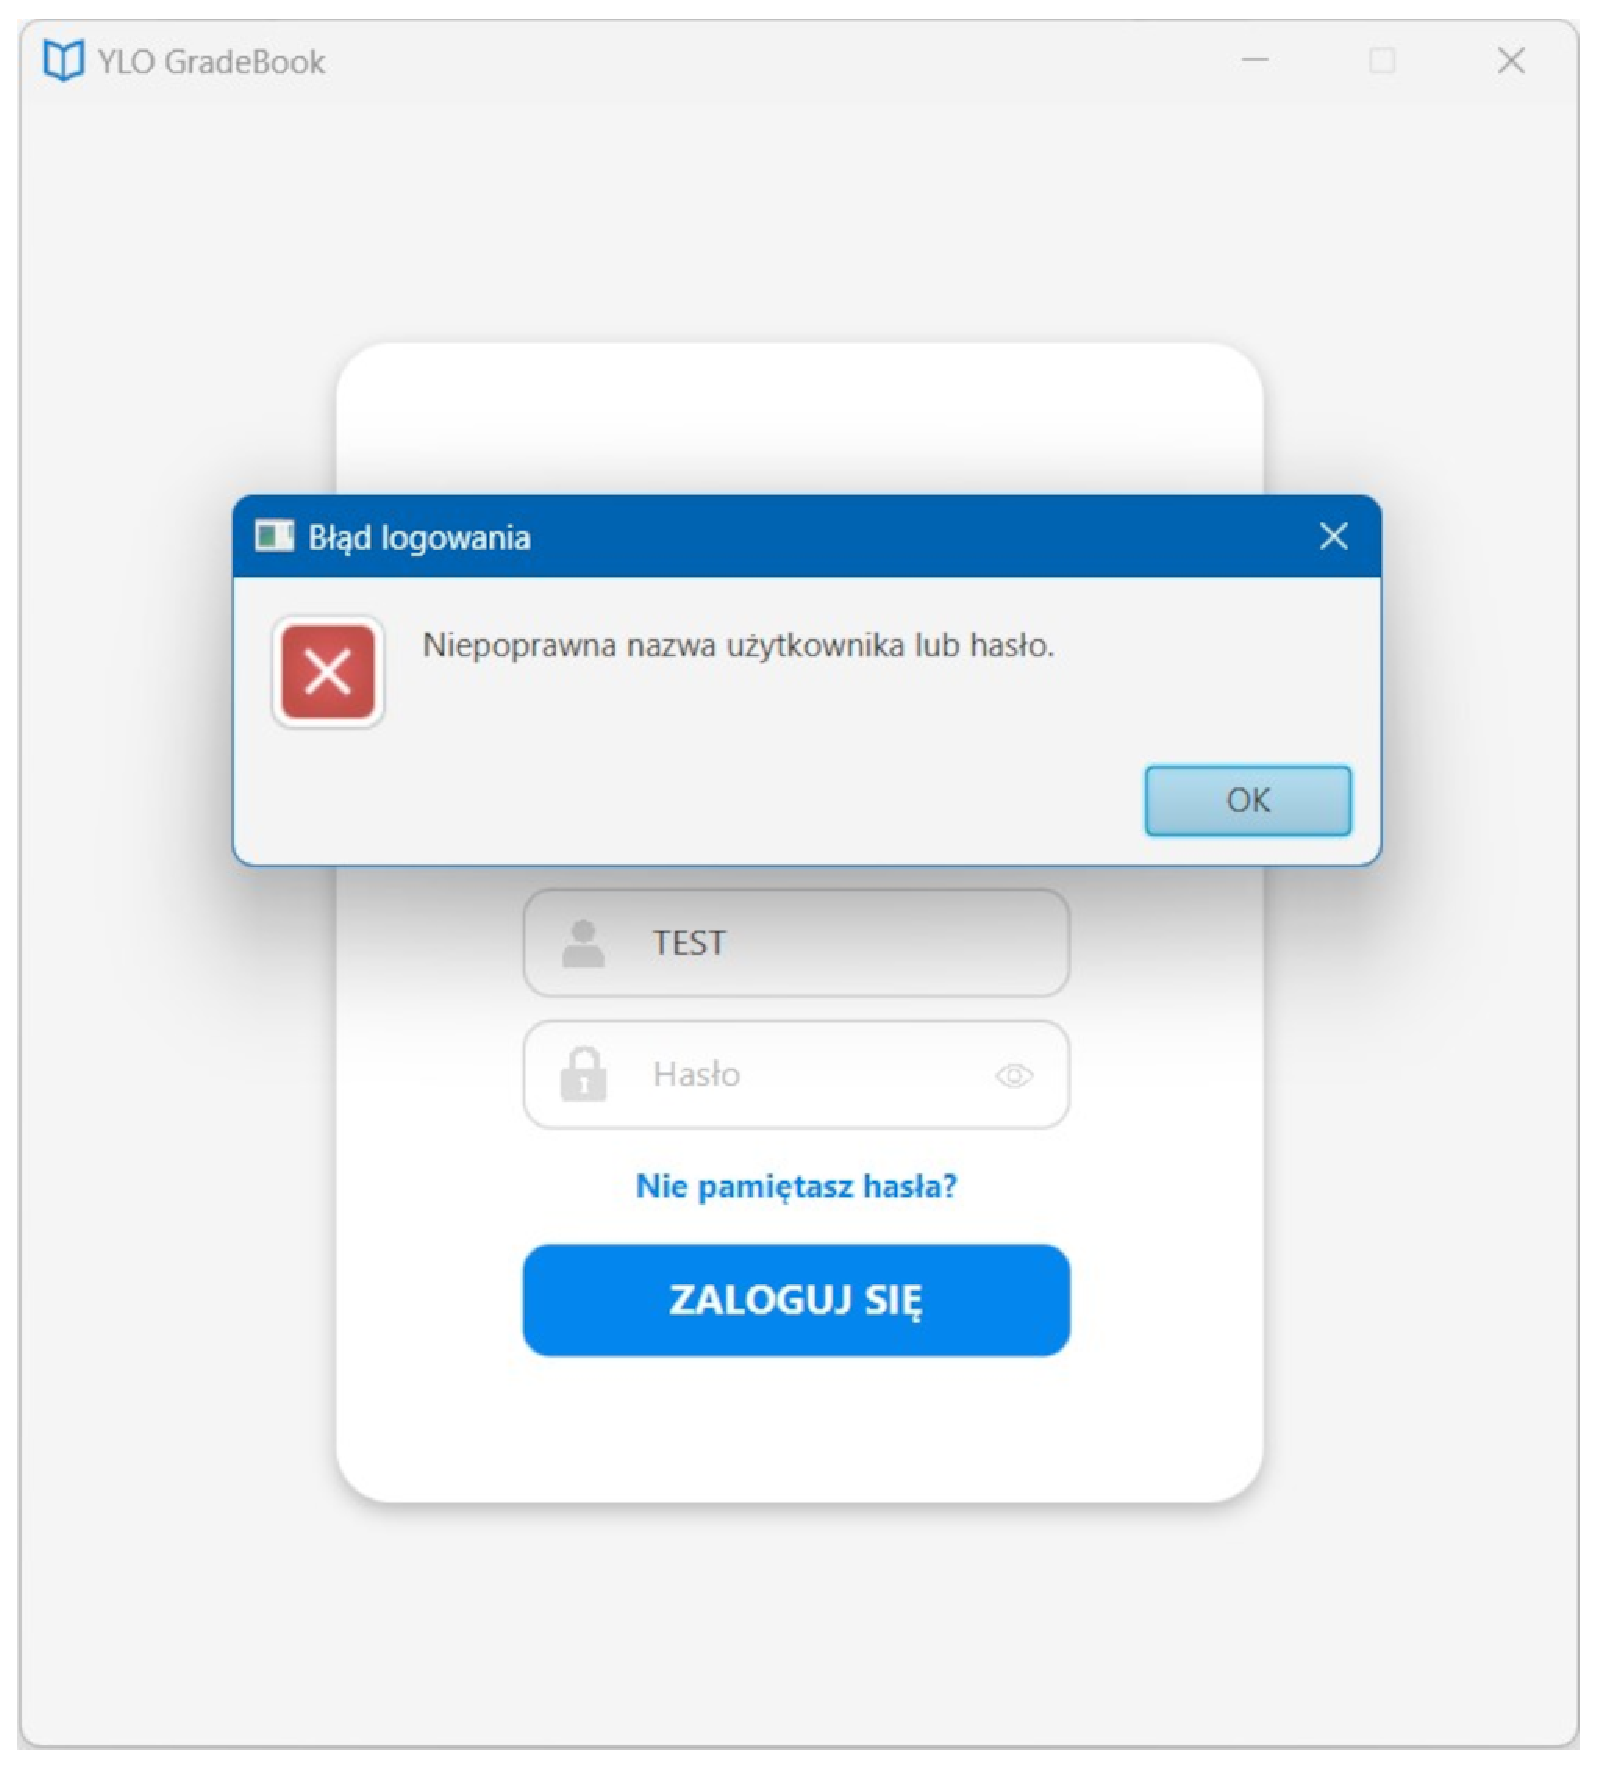
\includegraphics[width=0.9\textwidth]{figures/fig_0020.eps}
    \caption{Przykładowy alert systemowy — nieprawidłowe logowanie}
    \label{fig:alert}
\end{figure}

